\documentclass[10pt]{article}
\usepackage[margin=0.95in]{geometry}
\usepackage[T1]{fontenc}
\usepackage[utf8]{inputenc}
\usepackage{lmodern}
\usepackage{microtype}
\usepackage{amsmath,amssymb,mathtools,bm}
\usepackage{amsthm}
\usepackage{booktabs,tabularx,array,multirow,longtable}
\usepackage{graphicx}
\graphicspath{{figures/}}
\usepackage{listings,xcolor}
\usepackage[numbers,sort&compress]{natbib}
\usepackage[hidelinks]{hyperref}
\usepackage{xurl}
\usepackage{enumitem}
\usepackage{algorithm}
\usepackage{algpseudocode}
\usepackage{titlesec}
\usepackage{fancyhdr}
\usepackage{caption}
\usepackage{float}
\setlist{nosep,leftmargin=*}
\setlength{\parskip}{0.34em}
\setlength{\parindent}{0pt}
\setlength{\emergencystretch}{2em}
\renewcommand{\arraystretch}{1.12}
\urlstyle{same}
\setlength{\bibsep}{0.15\baselineskip}

\definecolor{Accent}{HTML}{164E63}
\definecolor{Accent2}{HTML}{0F766E}
\titleformat{\section}{\large\bfseries\color{Accent}}{\thesection}{0.6em}{}
\titleformat{\subsection}{\normalsize\bfseries\color{Accent2}}{\thesubsection}{0.6em}{}
\pagestyle{fancy}
\fancyhf{}
\lhead{CAVER: selective trusted verification for VLA post-training}
\rhead{\thepage}
\renewcommand{\headrulewidth}{0.3pt}

\theoremstyle{plain}
\newtheorem{theorem}{Theorem}[section]
\newtheorem{corollary}[theorem]{Corollary}
\theoremstyle{definition}
\newtheorem{assumption}{Assumption}
\renewcommand{\theassumption}{A\arabic{assumption}}
\theoremstyle{remark}
\newtheorem*{remark}{Remark}

\newcommand{\E}{\mathbb{E}}
\newcommand{\I}{\mathbb{I}}
\newcommand{\LCB}{\mathrm{LCB}}
\newcommand{\UCB}{\mathrm{UCB}}
\newcommand{\softmax}{\mathop{\mathrm{softmax}}}
\newcommand{\argmax}{\mathop{\mathrm{argmax}}}

\title{\textbf{CAVER: Calibrated Active Verification for Sample-Efficient Post-Training of Vision-Language-Action Policies}\\[0.35em]
\large Simulation-first LIBERO evidence for CAVER+FASR, with a gated PiPER Stage-F transfer plan}
\author{}
\date{June 2026}

\begin{document}
\maketitle

\begin{abstract}
CAVER studies a practical VLA post-training question: if only a small number of trusted executions are affordable, which attempted actions should be run, and which executed trajectories should be used to update the policy? The method samples several short candidate action chunks, uses a frozen future predictor as a cheap but imperfect hint, executes only one safe candidate, and logs exactly how that candidate was chosen.

The implementation is simulation-first. Stage 0 uses LIBERO as the trusted execution environment with the pretrained $\pi_{0.5}$ backbone from \texttt{openpi} and frozen GE-Sim from Genie Envisioner. Stage 1 is a planned transfer to PiPER hardware \citep{liao2025genie,genierepo2026}. The robot- or simulator-specific pieces are isolated behind four adapters: execution, provider input, safety checks, and task labeling.

The main Stage-0 empirical variant is CAVER+FASR: CAVER's provider-aware selection and calibration combined with failure-aware segment repair. Strict CAVER, which admits only confident full successful trajectories, is retained as the conservative base rule and ablation. In LIBERO, CAVER+FASR reaches held-out test success $0.237$ at $N=25$ with $796$ admitted demo items, versus $0.227$ with $1885$ demo items for vanilla $K=1$; at $N=50$ it reaches $0.240$ with $785$ demo items. A vanilla $K=1$+FASR control reaches only $0.223$ at $N=25$, so the completed evidence does not reduce to FASR on a single sampled chunk. The remaining fairness control, uniform $K=4$+FASR, is running and is not yet claimed as completed. These results support a simulation-stage selective-admission/sample-efficiency claim, while full real-robot sample efficiency remains the Stage-1 question. FASR requires reliable task-progress labels; if a task cannot provide them, the hardware method falls back to strict CAVER.
\end{abstract}


\begin{quote}
\textbf{Thesis in one sentence.} Use one frozen provider for scale, use one small budget of trusted executions for truth, and place an interface-general selective-verification layer between them, with one fully pinned Stage-0 LIBERO simulation instantiation and one fully pinned Stage-1 PiPER hardware instantiation in the implementation plan.
\end{quote}

\begin{table}[H]
\centering
\small
\caption*{What is completed and what is planned}
\begin{tabularx}{\linewidth}{@{}p{3.2cm}p{4.2cm}X@{}}
\toprule
Item & Status & What the reader should conclude \\
\midrule
Stage-0 LIBERO & Completed simulation evidence & CAVER+FASR is currently the strongest empirical variant. It modestly improves held-out test success over vanilla $K=1$ at $N=25$ and $N=50$ while admitting far fewer backend records. \\
Strict CAVER & Completed base ablation & Shows strong backend-data compression but does not clearly beat vanilla $K=1$ in raw held-out success. \\
FASR fairness controls & Partly completed, partly running & Vanilla $K=1$+FASR at $N=25$ does not explain the CAVER+FASR gain. Uniform $K=4$+FASR is the active control needed to separate CAVER selection from progress-label repair. \\
PiPER hardware & Planned Stage-F/Stage-1 path & No real-robot learning result is claimed. Stage F is the hardware-readiness gate before budgeted PiPER learning: shadow mode, safety, labeler, latency, and progress-label validation. \\
Scope of claim & Simulation-first, selective-admission claim & The current evidence supports selective-admission/sample-efficiency in LIBERO, not broad raw-success dominance or completed real-robot sample efficiency. \\
\bottomrule
\end{tabularx}
\end{table}

\begin{table}[H]
\centering
\small
\caption*{Plain-language guide to the main mathematical terms}
\begin{tabularx}{\linewidth}{@{}p{3.1cm}X@{}}
\toprule
Term & Meaning in this paper \\
\midrule
Decision context & One moment where the policy chooses the next short action chunk, not one low-level control tick. \\
Candidate chunk & One possible short action sequence. In CAVER and the matched uniform baseline, $K=4$ candidates are sampled and each has $H=4$ commands, about 0.4 s of motion. The vanilla baseline uses $K=1$. \\
Trusted execution & Actually running one selected candidate in LIBERO or on PiPER and measuring the task outcome. \\
Stage F & The hardware-readiness gate before budgeted PiPER learning. It includes no-motion shadow mode, safety validation, labeler validation, progress-label validation, and latency checks. \\
Provider & A frozen future predictor. GE-Sim gives cheap predicted futures; CAVER treats them as useful but fallible hints. \\
Selector & The rule that assigns probabilities to safe candidates and samples one to execute. \\
Propensity & The exact probability with which the executed candidate was selected. It is logged so later correction is auditable. \\
Calibrator & A small model that converts cheap features into a corrected value and uncertainty after seeing verified outcomes. \\
DR correction & A standard correction that combines the observed outcome of the executed candidate with the logged selection probability. It reduces bias from executing only one candidate. \\
Conservative score / LCB & The corrected value minus an uncertainty penalty. CAVER admits a trajectory to backend training only when this score is high enough. \\
FASR & Failure-aware segment repair. If a failed episode contains a short, verified-progress prefix, CAVER+FASR may admit that prefix as a repair segment instead of relabeling the whole failed episode as successful. \\
Online success & Success observed during the training-context collection episodes. It is useful for diagnostics, but it is not disjoint evaluation. \\
Held-out validation/test success & Success on disjoint LIBERO or PiPER evaluation episodes that are not admitted to training or calibrator fitting. \\
Admitted demo items & The training records actually passed into the unchanged backend. This can be far smaller than the number of executed contexts. \\
Primitive steps & Low-level action-step records inside admitted trajectories. \\
\bottomrule
\end{tabularx}
\end{table}


\begin{table}[H]
\centering
\small
\caption*{Locked design decisions}
\begin{tabularx}{\linewidth}{@{}p{3.4cm}p{3.6cm}X@{}}
\toprule
Decision point & Locked choice & Why it is locked \\
\midrule
Action backbone & Pretrained $\pi_{0.5}$ from \texttt{openpi} & Matches the public flow-based VLA stack and supports a direct comparison with flow-based real-only post-training \citep{pi052025,openpi2026repo}. \\
Method presentation & Interface-general modules $(\Gamma_{\mathrm{exec}},\Phi_{\Omega},S_{\mathrm{safe}},M_{\mathrm{task}})$ plus concrete Stage-0 LIBERO and Stage-1 PiPER instantiations & Keeps the scientific claim at the interface level while preserving one exactly reproducible simulation-first path and one exactly reproducible hardware transfer study. \\
Cheap future provider & Frozen GE-Sim from Genie Envisioner & Satisfies the preference for an off-the-shelf world model and keeps the paper about verification rather than training a new simulator \citep{liao2025genie,genierepo2026}. \\
Concrete trusted-execution stacks & LIBERO simulation in Stage 0; PiPER single-arm manipulation in Stage 1 & Makes the debugging and calibration stage concrete before the real study while keeping the eventual hardware transfer equally auditable. \\
Cheap utility head & Small 3-head MLP trained on Stage-0 data plus the shared Stage-1 seed set & Avoids training a world model from scratch while still providing a task-specific scalar for selection. \\
Executed-update backend & $\pi$-StepNFT-style executed-trajectory fine-tuning & Fits flow-based VLAs without requiring tractable action likelihoods or a learned critic \citep{wang2026pistepnft,pistepnftrepo2026}. \\
Execution safety & Shared deterministic safety shield plus runtime abort rules & Prevents unsafe candidate chunks from reaching hardware and makes the real study auditable across methods. \\
Selector learning & No online selector-parameter learning in the main method & Keeps the verification rule fixed and auditable. The selector form and coefficients are frozen after Stage 0; only the utility inputs refresh. \\
Main admission rule & CAVER+FASR for the Stage-0 empirical main variant; strict CAVER as the conservative base ablation & FASR addresses sparse-success regimes by preserving successes and adding only short verified-progress repair segments from failures, without changing the backend objective. \\
Frozen features & Provider and calibration features come from frozen encoders & Keeps the cheap-feature space fixed while policy adaptation touches only LoRA modules in the action head. \\
World-model baseline & WoVR via RLinf & Gives the strongest world-model-heavy comparison already supported in a public RL stack \citep{jiang2026wovr,rlinfrepo2026}. \\
\bottomrule
\end{tabularx}
\end{table}

\section{Introduction}
World models, verifier scores, and large VLA backbones have made it easy to generate many candidate robot behaviors together with cheap predicted futures and cheap reward-like signals. At the same time, recent post-training work keeps returning to the same bottleneck: the hard part is not producing \emph{more} feedback, but producing feedback that is trustworthy enough to update the policy \citep{tan2025riptvla,jiang2026wovr,li2025worldmodelbench}. World-VLA-Loop, WoVR, TGRPO, NORA-1.5, and VLA-RFT all illustrate versions of the same tension. Learned simulators and reward proxies can provide scale, but simulator hallucination, compounding error, sparse success labels, and proxy exploitation make naive optimization brittle \citep{liu2026worldvlaloop,jiang2026wovr,chen2025tgrpo,hung2025nora15,li2025vlarft}.

This paper takes that tension as the central problem. Let $M$ be a large pool of cheap imagined or proxy-scored candidates, and let $N \ll M$ be a much smaller set of trusted executions. The scientific question is not ``which reward function should we use?'' It is: \emph{how should a small trusted-execution budget be allocated and converted into a reliable policy-improvement signal?} In Stage 0 the trusted executor is LIBERO simulation; in Stage 1 it is the PiPER robot.

The theory here is deliberately narrow. It justifies a \emph{context-level} verification rule conditional on the stream of decision contexts that actually occurs; it does not claim a full episodic policy-improvement guarantee after online backbone updates.

This question is especially sharp for flow-based VLAs. The current public \texttt{openpi} implementation supports $\pi_{0.5}$ with a flow-matching action head. Flow-based action generation makes standard likelihood-ratio RL awkward, critic learning can be heavy, and a practical first-paper route is a critic-free, likelihood-free executed-trajectory update such as $\pi$-StepNFT \citep{openpi2026repo,wang2026pistepnft}. Accordingly, the method keeps the backbone fixed at $\pi_{0.5}$ and keeps the executed-update backend close to that path rather than turning the proposal into a new flow-RL optimizer paper.

A second key design choice is to treat the world model as a \emph{frozen provider} rather than a new training target. The mainline method therefore uses a frozen off-the-shelf provider, with GE-Sim from Genie Envisioner as the primary choice because the public repository exposes code, released weights for GE-Sim, and example inference scripts that consume images, camera intrinsics/extrinsics, and action arrays \citep{liao2025genie,genierepo2026}. This keeps the contribution focused on verification and makes the approach transferable across backbones and world models.

The claim is deliberately modest. CAVER is not presented as a new end-to-end RL algorithm for all flow-based VLAs. It is a \emph{training-time selective-verification layer}. Relative to ALOE, which studies action-level off-policy evaluation from logged VLA data, CAVER adds an online data-collection decision: it chooses which cheap candidate to verify in the first place, then uses that verified outcome to decide which executed trajectories deserve an update \citep{yang2026aloe}. Relative to WoVR and World-VLA-Loop, CAVER does not ask the world model to become increasingly reliable through policy/world co-training; it instead treats the world model as fallible and spends trusted interaction only where it is most valuable \citep{jiang2026wovr,liu2026worldvlaloop}. Relative to direct executed-trajectory post-training, it asks whether the same trusted budget can be used more intelligently.

\paragraph{Contributions.}
\begin{enumerate}
    \item A \textbf{problem formulation} for VLA post-training under limited trusted verification, in which a frozen off-the-shelf world-model provider produces cheap predicted futures while trusted execution supplies the label.
    \item A \textbf{two-layer CAVER specification}: an interface-general method defined by an execution adapter, provider adapter, safety shield, and verified labeler, together with concrete Stage-0 LIBERO and Stage-1 PiPER instantiations.
    \item A \textbf{roundwise selective-verification algorithm} with exact feature definitions, exact selector behavior, exact roundwise data flow, explicit frozen-vs-trainable components, failure-aware admission through CAVER+FASR, and an implemented-path update backend.
    \item A \textbf{reproducible implementation and current Stage-0 result} using $\pi_{0.5}$, GE-Sim, LIBERO, and $\pi$-StepNFT, together with a clearly delimited Stage-1 PiPER transfer plan.
\end{enumerate}

\section{Related work and positioning}\label{sec:related}
CAVER sits at the intersection of four lines of work: executed-trajectory post-training for flow-based VLAs, world-model-assisted VLA learning, off-policy evaluation under limited trusted feedback, and safety-aware robot deployment. This section makes the comparison explicit because the method is an integration paper: the individual statistical and systems components are familiar, but the combination is targeted at a narrow gap in VLA post-training.

\subsection{Executed-trajectory post-training for VLAs}
A first family updates a VLA directly from executed trajectories. RIPT-VLA and action-chunked PPO variants use online execution feedback for policy improvement, while TGRPO applies group-relative policy optimization ideas to VLA fine-tuning \citep{tan2025riptvla,wang2025actionchunkppo,chen2025tgrpo}. These methods are important because they show that closed-loop post-training can improve manipulation policies, but they either require action likelihoods or critic/advantage machinery that is not the simplest route for a flow-matching backbone such as $\pi_{0.5}$. $\pi$RL directly addresses this issue by converting flow-based VLA generation into RL-compatible stochastic processes through Flow-Noise and Flow-SDE \citep{chen2025pirl}. CAVER deliberately does not compete as a new policy-gradient optimizer. It keeps the executed-update backend close to $\pi$-StepNFT, a critic- and likelihood-free method designed for flow-based VLAs, and asks whether better verification and admission can feed that same backend more useful records \citep{wang2026pistepnft,pistepnftrepo2026}.

\subsection{World models as simulators, evaluators, and preference generators}
A second family uses learned dynamics or video prediction models to obtain cheap scale. World-VLA-Loop co-trains a world model and VLA policy, while WoVR uses world models as reliable simulators for post-training and explicitly addresses hallucination and long-horizon error accumulation \citep{liu2026worldvlaloop,jiang2026wovr}. VLA-RFT similarly uses a data-driven world simulator with verified reward signals, and Sword studies robustness of world-model simulators under style and initial-state perturbations \citep{li2025vlarft,gao2026sword}. Other work uses world models primarily as evaluators: NORA-1.5 constructs preference data from world-model and action-based rewards, and Cosmos Policy exposes future-state value signals useful for planning-style scoring \citep{hung2025nora15,kim2026cosmospolicy}. CAVER is more conservative than these world-model-heavy approaches. It uses GE-Sim as a frozen provider for short-horizon features, but it does not treat imagined rollouts as ground truth and does not update the backbone directly from unverified provider futures. The trusted label still comes from LIBERO execution in Stage 0 or planned PiPER execution in Stage 1.

\subsection{Off-policy evaluation, doubly robust correction, and high-confidence improvement}
The statistical layer in CAVER draws from contextual-bandit and reinforcement-learning off-policy evaluation. Doubly robust estimators combine a direct model with inverse-propensity correction, and the RL extension of Jiang and Li shows why exact propensities plus a useful model can reduce variance relative to pure importance weighting \citep{dudik2011dr,jiang2016doubly}. High-confidence policy-improvement and safe policy-improvement methods add conservative decision rules around such estimates \citep{thomas2015hcpi,laroche2019spibb}. CAVER does not claim these estimators are new. Its use of DR is narrower: each decision context has a small menu of safety-approved candidate chunks, one candidate is sampled with an exact logged propensity, and the resulting trusted label is used to correct candidate-level utilities for the next admission/selection step. This is also distinct from ALOE, which frames VLA post-training as action-level off-policy evaluation from logged VLA chunks; CAVER adds the online or batch data-collection decision of which candidate to verify before execution \citep{yang2026aloe}.

\subsection{Safety-aware VLA deployment and verified labels}
Hardware VLA learning cannot rely only on objective functions. SAFE and SafeVLA motivate failure detection and constraint-aware deployment for VLA systems \citep{gu2025safe,zhang2025safevla}. CAVER's safety shield is not the algorithmic novelty, but it is essential for a fair and auditable real-robot study: every method shares the same deterministic pre-execution filter, runtime abort rules, and safety-abort accounting. This also clarifies the status of CAVER+FASR. FASR does not relabel failed episodes as successes. It admits only short progress-verified repair segments, and only when the progress labeler is reliable. If Stage-F PiPER shadow-mode checks cannot validate those progress labels, the hardware pilot falls back to strict CAVER.

\subsection{Summary of closest neighbors}
\begin{table}[H]
\centering
\small
\caption{Closest related methods and the specific gap CAVER targets. CAVER's claim is not that these ingredients are individually new; it is that a fixed-backend VLA post-training stack benefits from calibrated selective verification and explicit admission under a small trusted-execution budget.}
\begin{tabularx}{\linewidth}{@{}p{2.3cm}p{3.3cm}p{3.2cm}X@{}}
\toprule
Method family & Representative methods & Primary learning signal & Difference from CAVER \\
\midrule
Executed-trajectory post-training & $\pi$-StepNFT, RIPT-VLA, TGRPO, action-chunked PPO, $\pi$RL \citep{wang2026pistepnft,tan2025riptvla,chen2025tgrpo,wang2025actionchunkppo,chen2025pirl} & Executed rollouts, group advantages, critic/likelihood machinery, or flow-specific RL & CAVER keeps the executed-sample backend fixed and changes only verification allocation and data admission. \\
World-model-heavy post-training & WoVR, World-VLA-Loop, VLA-RFT, Sword \citep{jiang2026wovr,liu2026worldvlaloop,li2025vlarft,gao2026sword} & Imagined rollouts or learned simulator feedback & CAVER treats the provider as fallible; imagined futures provide features, not direct backbone training labels. \\
World-model preference/evaluation & NORA-1.5, Cosmos Policy \citep{hung2025nora15,kim2026cosmospolicy} & Preference rewards or future-state values from a model & CAVER calibrates cheap scores against trusted outcomes and uses them for selection/admission rather than direct DPO or planning claims. \\
Off-policy evaluation and safe improvement & ALOE, DR/OPE, HCPI, SPIBB \citep{yang2026aloe,dudik2011dr,jiang2016doubly,thomas2015hcpi,laroche2019spibb} & Logged data, propensities, value estimates, confidence bounds & CAVER applies this logic to VLA candidate menus and decides what to verify before execution. \\
Safety-aware deployment & SAFE, SafeVLA \citep{gu2025safe,zhang2025safevla} & Failure detection or constraints & CAVER uses safety as a shared execution guardrail, not as the main learning contribution. \\
\bottomrule
\end{tabularx}
\label{tab:related_work}
\end{table}

\section{Scope and explicit design choices}
This section states the design choices that make the proposal both general at the method level and concrete at the implementation level.

\subsection{What this paper is and is not}
This is a \textbf{selective-verification paper}. It is not a full policy-gradient method for flow-based VLAs, it is not a new critic-learning paper, and it is not a world-model-training paper. The main contribution is also not doubly robust estimation by itself; that machinery is borrowed. The contribution claimed here is the \emph{integration}: exact-propensity online verification allocation plus conservative/failure-aware admission into an unchanged executed-sample backend under a strict matched-budget protocol. In the current formulation, strict CAVER is the conservative base rule, and CAVER+FASR is the main Stage-0 empirical variant. The paper asks whether a small trusted-execution budget can produce a better learning signal than either direct executed-trajectory post-training or direct imagined-experience training. Natural extensions such as a $\pi$RL-style Flow-SDE policy-gradient backend, learned online selector policies, or multi-provider disagreement modeling are future work rather than part of the present claim.

\begin{table}[H]
\centering
\small
\caption*{Names of the CAVER variants used in this paper}
\begin{tabularx}{\linewidth}{@{}p{3.2cm}p{4.2cm}X@{}}
\toprule
Variant & Admission rule & Role in the paper \\
\midrule
Strict CAVER & Admit only full successful executed trajectories whose lower confidence bound exceeds the threshold. & Conservative base rule and backend-data-efficiency ablation; not the strongest raw-success variant. \\
CAVER+FASR & Preserve full successful trajectories and add only short verified-progress repair segments from failed episodes when the task progress label is reliable. & Main current Stage-0 empirical variant. It does not relabel whole failed episodes and does not change the backend objective. \\
Uniform $K=4$ & Sample one of four safe candidates uniformly and admit every executed trajectory to the same backend. & Matched candidate-wrapper baseline. \\
Vanilla $K=1$ & Sample and execute a single candidate without the $K=4$ wrapper. & Strong pressure-test baseline that must remain in the main comparison. \\
\bottomrule
\end{tabularx}
\end{table}

\subsection{What is general and what is instantiated}
CAVER's scientific claim is not tied to PiPER-specific joint commands. At the method level, the pipeline is defined by four interfaces:
\[
\tilde a^{\pi} \xrightarrow{\Gamma_{\mathrm{exec}}} a \xrightarrow{S_{\mathrm{safe}}} \nu_r \xrightarrow{\text{execute}} \text{episode trace} \xrightarrow{M_{\mathrm{task}}} Y,
\qquad
 a \xrightarrow{\Phi_{\Omega}} \tilde a^{\Omega} \xrightarrow{\mathcal T_{\Omega}} \hat I \xrightarrow{V_{\omega},f_{\psi}} (\hat v,\hat\sigma,\mu,\sigma).
\]
Only four modules are robot- or simulator-specific: the execution adapter $\Gamma_{\mathrm{exec}}$, the safety shield $S_{\mathrm{safe}}$, the provider adapter $\Phi_{\Omega}$, and the verified labeler $M_{\mathrm{task}}$. The staged study instantiates them twice. In Stage 0, LIBERO supplies simulator execution, finite/shape/magnitude candidate validity checks, a LIBERO-to-GE-Sim compatibility map, and the simulator task-success labeler. In Stage 1, PiPER supplies joint/gripper execution, a PiPER URDF-based safety shield, a PiPER-to-GE-Sim compatibility map, and a marker-based geometric labeler. Porting CAVER to another robot changes those modules and the local configs, but it does \emph{not} change selector scoring, exact propensity logging, doubly robust correction, calibrator fitting, or the StepNFT-style executed-update backend.

\subsection{Why the mainline uses an off-the-shelf world model}
The mainline method uses a frozen off-the-shelf provider because this is the cleanest way to isolate the proposed contribution. A new world model would introduce another training problem, another set of hyperparameters, and another source of failure. GE-Sim is therefore the primary provider because its public repository includes released GE-Sim weights, an example inference path, and explicit instructions for passing images, camera intrinsics/extrinsics, and actions into the simulator \citep{genierepo2026}. The proposal also keeps a local lightweight provider only as a \emph{contingency}; see Appendix~\ref{app:contingency}. Replacing GE-Sim in a future study would change $\Phi_{\Omega}$ and the provider-specific input bundle, not the selective-verification logic itself. The paper therefore generalizes across interfaces, not by claiming that every robot stack is already validated empirically.

\subsection{Why the update backend is executed-sample \texorpdfstring{$\pi$-StepNFT}{pi-StepNFT}}
Critic-free, likelihood-free fine-tuning is the most direct practical route on $\pi_{0.5}$, and the public ecosystem supports that route. The open-source $\pi$-StepNFT code is public and is already framed as a critic-and-likelihood-free method for flow-based VLAs \citep{wang2026pistepnft,pistepnftrepo2026}. This proposal therefore uses the released $\pi$-StepNFT objective as the real-only baseline and as the backbone-update backend inside CAVER. In the main comparison, CAVER keeps the StepNFT loss, optimizer, LoRA target modules, batch size, gradient clip, and update schedule unchanged. It differs only in how candidate chunks are scored before execution, which executed contexts are admitted to training, and which exact propensities are logged for doubly robust correction.

\subsection{How the selector is fixed yet still improves over rounds}
The \textbf{selector functional form is frozen after Stage 0}. Its scalar coefficients, temperature, and exploration floor are tuned once in Stage 0 and never learned online. However, its value and uncertainty inputs are allowed to refresh round-by-round through the latest calibrated utility model. In other words, the selector does \emph{not} have trainable online parameters, but it can still make better decisions over time because it reads the newest corrected utility estimates.

\subsection{Frozen features and trainable components}
The cheap-feature space does \textbf{not} move while the policy is being updated. The encoders used to build $e_{r,c}$, $q_{r,c,k}$, and therefore $z_{r,c,k}$ are frozen throughout Stage 1. Only LoRA modules are updated inside the action head used for the final policy improvement. Here \emph{LoRA} means \emph{low-rank adaptation}: small trainable low-rank matrices are inserted into a frozen pretrained network so that most original weights remain fixed.

\section{Problem setup and notation}
This section introduces symbols, but the operational idea is simple. A run is split into rounds. In each decision context, the policy proposes a few short action chunks, CAVER selects one safe chunk to verify, and the outcome is used after the round to update the calibrator and possibly the policy backend. The long notation table is a reference table; first-time readers can skip it and use the plain-language guide above.

\subsection{Roundwise decision process}
Training proceeds in rounds $r=1,2,\dots,R$. In the planned Stage-1 PiPER study, each online training run is task-specific: one run fine-tunes one copy of the common seed-warmed checkpoint on exactly one physical task, and task averages are formed only after those per-task runs finish. The completed Stage-0 LIBERO experiments instead use balanced multi-family proxy runs so that one simulation run can cover all five proxy families under a shared budget curve. A \textbf{decision context} is a chunk boundary inside an episode, not an individual low-level control step. Each episode allows at most four decision contexts.

A \textbf{round} is operationally fixed to
\[
B_{\mathrm{round}}=25
\]
\emph{counted training contexts} on a single task. A counted context is either (i) one safety-approved candidate that is actually executed on hardware or in simulation, or (ii) one ``no safe candidate'' event that is logged as \texttt{safety\_abort} and charged to the budget even though no motion is executed. Because all main budgets satisfy $N\in\{25,50,100,200\}$, every run has exactly
\[
R=N/B_{\mathrm{round}}\in\{1,2,4,8\}
\]
rounds and there is no partial final round in the main experiments. Within one round, the backbone policy $\pi_{\theta_r}$, the selector $\nu_r$, the previous-round prediction model $m_{r-1}$, and the safety shield are frozen. Only after the round closes are the calibrator and, if triggered, the LoRA modules updated.

This roundwise convention makes the theory--protocol link explicit. The potential outcome $Y_{r,c}(k)\in\{0,1\}$ means the eventual episode-success label that would be observed in round $r$ if candidate $k$ were executed at context $c$ and the remainder of the episode were completed by the frozen continuation policy $\pi_{\theta_r}$. The observed label is $Y_{r,c}=Y_{r,c}(A_{r,c})$.

\subsection{Method-level interfaces and current instantiation}
The method itself is written around two deterministic translation steps and two deterministic trust layers:
\[
\tilde a^{\pi}_{r,c,k}\xrightarrow{\Gamma_{\mathrm{exec}}} a_{r,c,k}\xrightarrow{S_{\mathrm{safe}}}\text{trusted execution},
\qquad
 a_{r,c,k}\xrightarrow{\Phi_{\Omega}} \tilde a^{\Omega}_{r,c,k}\xrightarrow{\mathcal T_{\Omega}} \hat I_{r,c,k,1:H}.
\]
The first map, $\Gamma_{\mathrm{exec}}$, turns raw backbone outputs into a safety-checkable execution-space chunk for the chosen trusted execution environment. The second map, $\Phi_{\Omega}$, turns that same execution chunk into the frozen provider's conditioning format. The trust layers are (i) the hard safety shield $S_{\mathrm{safe}}$, which determines which candidates may be executed at all, and (ii) the verified labeler $M_{\mathrm{task}}$, which turns the executed episode into a trusted binary outcome. In the present study, Stage 0 instantiates these modules with a LIBERO execution adapter, simulator-side validity checks for finite tensors, expected chunk shape, and broad action magnitude bounds, a LIBERO-to-GE-Sim compatibility map, and the simulator task labeler; Stage 1 instantiates them with a PiPER joint/gripper adapter, a PiPER-to-GE-Sim compatibility map, a PiPER URDF-based hard filter, and a marker-based geometric labeler. The selector, DR correction, calibrator, and StepNFT-style update backend do not depend on which concrete robot or simulator instantiates those four modules.

\subsection{Reference notation table}
{\footnotesize
\refstepcounter{table}\label{tab:master_notation}
\noindent\textbf{Table~\thetable.} Reference notation table used throughout the proposal. It is included for auditability; it is not required for a first pass through the method.
\par\smallskip
\setlength{\LTleft}{0pt}
\setlength{\LTright}{0pt}
\begin{longtable}{@{}>{\raggedright\arraybackslash}p{3.25cm}>{\raggedright\arraybackslash}p{2.55cm}>{\raggedright\arraybackslash}p{8.35cm}@{}}
\toprule
Symbol & Name & Exact meaning in this proposal \\
\midrule
\endfirsthead
\multicolumn{3}{@{}l@{}}{\emph{Table~\thetable{} continued.}}\\
\toprule
Symbol & Name & Exact meaning in this proposal \\
\midrule
\endhead
$r$ & round index & One collection-and-update block of exactly $B_{\mathrm{round}}=25$ counted training contexts. Stage 1 is task-specific; completed Stage 0 uses balanced multi-family proxy manifests. \\
$c$ & context index & Decision-context index within the current round and episode. \\
$B_{\mathrm{round}}$ & round size & Fixed at 25 counted training contexts per round in both Stage 0 and Stage 1. \\
$h_{r,c}$ & observation bundle & Policy-view observations, optional provider-only auxiliary views, robot state, and any calibration metadata required by the concrete instantiation. \\
$g_{r,c}$ & instruction & Task-language string for the current episode. \\
$s^{\mathrm{prop}}_{r,c}$ & robot state & Current robot state passed to the policy and execution adapter; in the current study this is joint position/velocity plus gripper state. \\
$e_{r,c}$ & frozen context embedding & Context embedding produced by the frozen encoder $E_{\phi}^{\mathrm{frz}}$. \\
$E_{\phi}^{\mathrm{frz}}$ & frozen context encoder & The frozen $\pi_{0.5}$ context encoder used to form $e_{r,c}$ and start-state embeddings. \\
$\pi_{\theta_r}$ & backbone policy & Frozen $\pi_{0.5}$ backbone used during data collection of round $r$. \\
$\theta_{\mathrm{roll}}$ & rollout checkpoint & Frozen policy parameters that originally generated the executed trajectories currently being optimized by StepNFT. \\
$K$ & candidates per context & Fixed at $K=4$ for CAVER and the matched uniform baseline; vanilla $K=1$ is reported as a stricter real-only baseline. \\
$H$ & chunk horizon & Fixed at $H=4$ executed commands per candidate chunk. \\
$\Delta t$ & control interval & Fixed at $\Delta t=0.1$ s, i.e. 10 Hz chunk execution. \\
$d_{\mathrm{exec}}$ & execution dimension & Per-step dimension of one execution-space command after $\Gamma_{\mathrm{exec}}$; the current study uses $d_{\mathrm{exec}}=7$. \\
$d_{\Omega}$ & provider dimension & Per-step dimension of one provider-conditioning vector after $\Phi_{\Omega}$; the current study uses $d_{\Omega}=16$. \\
$\tilde a^{\pi}_{r,c,k}$ & raw backbone chunk & The $k$th sampled raw chunk from $\pi_{\theta_r}$ before robot-specific execution conversion. \\
$a_{r,c,k}$ & execution-space chunk & The $k$th $H\times d_{\mathrm{exec}}$ chunk after $\Gamma_{\mathrm{exec}}$; this is the command actually handed to the safety shield and, if selected, to the robot bridge. \\
$\tilde a^{\Omega}_{r,c,k}$ & provider-space chunk & The $H\times d_{\Omega}$ chunk passed to the frozen provider after $\Phi_{\Omega}$. \\
$\Gamma_{\mathrm{exec}}$ & execution adapter & Deterministic map from raw backbone outputs and current robot state into safety-checkable execution commands; the current-study alias is $\Gamma_{\pi\rightarrow p}$. \\
$\Phi_{\Omega}$ & provider adapter & Deterministic map from execution-space chunks into the provider's input action format; the current-study alias is $\Phi_{\mathrm{GE}}$. \\
$S_{\mathrm{safe}}$ & safety shield & Deterministic hard constraint checker applied before execution. \\
$M_{\mathrm{task}}$ & verified labeler & Deterministic task-success measurement rule applied after executed episodes. \\
$\Gamma_{\pi\rightarrow p}$ & current-study execution adapter & Concrete PiPER instantiation of $\Gamma_{\mathrm{exec}}$. \\
$\Phi_{\mathrm{GE}}$ & current-study provider adapter & Concrete GE-Sim instantiation of $\Phi_{\Omega}$. \\
$\tilde a^{\mathrm{GE}}_{r,c,k}$ & current-study provider chunk & GE-Sim action array written by the present PiPER-to-GE-Sim compatibility map. \\
$\hat I_{r,c,k,1:H}$ & predicted future outputs & The frozen provider's predicted outputs for candidate $k$ across the $H$-step horizon. \\
$\hat I^{\mathrm{head}}_{r,c,k,H}$ & current-study summary frame & Final predicted head-view frame used as the cheap future summary in the present GE-Sim instantiation. \\
$F_{\rho}^{\mathrm{frz}}$ & frozen future encoder & Frozen visual encoder applied to the summary provider output. \\
$R$ & random projection & One fixed Gaussian projection that maps the pooled future-frame feature to 64 dimensions. \\
$q_{r,c,k}$ & future embedding & 64-dimensional projected feature extracted from the provider summary output. \\
$\phi_a(\cdot)$ & action encoder & Flattened standardized action representation defined in Step 3. \\
$V_{\omega}^{(b)}$ & bootstrap head & The $b$th head of the 3-head cheap utility predictor. \\
$\hat v_{r,c,k}$ & raw proxy utility & Mean cheap scalar utility estimate across the 3 bootstrap heads. \\
$\hat \sigma^{\mathrm{pre}}_{r,c,k}$ & proxy uncertainty & Standard deviation across the bootstrap heads of $V_{\omega}$. \\
$\mathcal D_{\mathrm{seed}}$ & warm-start seed set & The fixed fully verified set used before round 1 to create the common seed-warmed checkpoint and fit CAVER's initial calibrator $f_{\psi_0}$. \\
$f_{\psi_0}$ & initial calibrator & Calibrator fit once on $\mathcal D_{\mathrm{seed}}$ before round 1; later rounds refit $f_{\psi_r}$. \\
$\mathcal I_V$ & proxy-training index set & All Stage-0 train-split tuples plus the shared seed-real tuples used to fit the utility head. \\
\(\mathcal T^{\mathrm{seed}}_{\mathrm{S0}}\), \(\mathcal T^{\mathrm{train}}_{\mathrm{S0}}\), \(\mathcal T^{\mathrm{val}}_{\mathrm{S0}}\), \(\mathcal T^{\mathrm{test}}_{\mathrm{S0}}\) & Stage-0 partitions & Disjoint Stage-0 seed, training, validation, and audit-test template lists defined once before any tuning. \\
$J_{\mathrm{S0}}$ & selector-selection score & Scalar Stage-0 model-selection score used only to choose frozen selector coefficients. \\
$b_{r,c,k}$ & base feature vector & Cheap feature vector before novelty is appended. \\
$\mathcal B_{\mathrm{hist}}$ & executed-history reservoir & FIFO reservoir of executed base features used for novelty. \\
$D_{r,c,k}$ & within-context disagreement & Mean action-space distance from candidate $k$ to the other $K-1$ candidates in the same context. \\
$N_{r,c,k}$ & novelty & Nearest-neighbor distance from $b_{r,c,k}$ to the executed-history reservoir. \\
$z_{r,c,k}$ & final cheap feature vector & $z_{r,c,k}=[b_{r,c,k},N_{r,c,k}]$. \\
$s_{r,c,k}$ & selector score & Pre-softmax frozen-form selector score for candidate $k$ in context $(r,c)$. \\
$\nu_r(k\mid c)$ & verification selector & Frozen-form stochastic selector over the $K$ candidates in round $r$. \\
$p_{r,c,k}$ & propensity & Exact logged selection probability $\nu_r(k\mid c)$. \\
$\mathcal K^{\mathrm{safe}}_{r,c}$ & safe candidate set & Indices of candidates that pass the deterministic pre-execution safety shield. \\
$m_{r-1}(z)$ & previous-round prediction model & Cheap utility estimate available before round $r$ begins; in statistics this is often called a nuisance model. \\
$\tilde y^{\mathrm{DR}}_{r,c,k}$ & DR pseudo-outcome & Doubly robust corrected utility target for candidate $k$. \\
$\mathcal D^{\mathrm{tuple}}_{\le r}$ & accumulated tuple set & All non-aborted candidate tuples from verified contexts up to and including round $r$. \\
$f_{\psi_r}$ & calibrator & Mean/scale predictor refitted after collecting round-$r$ trusted execution data. \\
$\mu_r(z),\sigma_r(z)$ & corrected utility & The calibrator's corrected mean and input-dependent uncertainty scale. \\
$\bar\mu_r(z)$ & clipped probability diagnostic & $\bar\mu_r(z)=\mathrm{clip}(\mu_r(z),0,1)$ used only for probability-style metrics. \\
$\LCB_r(z)$ & conservative utility & $\mu_r(z)-\kappa\sigma_r(z)$. \\
\(\mathcal M_{\le r}^{+}\), \(\mathcal M_{\le r}^{-}\), \(\mathcal M_{\le r}^{0}\) & cumulative buffers & Positive, negative, and abstain executed-trajectory buffers used from rounds $1{:}r$. \\
$\mathcal M_{\le r}^{\mathrm{rep}}$ & FASR repair buffer & Verified-progress prefix segments from failed episodes; empty when running strict CAVER. \\
$\mathcal P_{\le r}$ & cumulative pair set & Positive--negative trajectory pairs built from the cumulative buffers after round $r$. \\
$q_f(t)$ & task progress label & Continuous progress score for task family $f$ at step or chunk index $t$, measured by the trusted environment rather than GE-Sim. \\
$t^*,\Delta q^*$ & FASR endpoint/gain & Best verified-progress prefix endpoint and its progress gain relative to the start of the failed episode. \\
$\mathcal F_{\mathrm{hard}}$ & FASR-eligible families & Task families where failed episodes may contain useful verified-progress prefixes. \\
$\delta_{\mathrm{prog}},\delta_{\mathrm{reg}}$ & FASR gates & Minimum required progress gain and maximum allowed pre-endpoint regression for repair admission. \\
$z^{\mathrm{exec}}_{r,c}$ & evaluation feature & Method-agnostic executed feature vector used by the common post-hoc calibration predictor. \\
$g_{\mathrm{eval}}$ & diagnostic predictor & Common post-hoc probability predictor used only to compute cross-method Brier/ECE. \\
$N_{\mathrm{val}}^{\mathrm{ctx}},N_{\mathrm{test}}^{\mathrm{ctx}}$ & evaluation interaction counts & Decision-context counts consumed by validation and test episodes; these are simulated in Stage 0 and real on PiPER in Stage 1. \\
$N_{\mathrm{total}}$ & total Stage-1 real interaction count & $120+N+N_{\mathrm{val}}^{\mathrm{ctx}}+N_{\mathrm{test}}^{\mathrm{ctx}}$ for the PiPER study. \\
$\mathrm{StdNorm}(\cdot)$ & standardizer & Per-dimension $z$-score normalization using Stage-0 train-split statistics only. \\
$\mathrm{vec}(\cdot)$ & vectorizer & Row-major flattening of one $H\times d_{\mathrm{exec}}$ action chunk into a length-$Hd_{\mathrm{exec}}$ vector. \\
$\mathrm{NN}_1(\cdot;\mathcal B)$ & nearest neighbor & Euclidean nearest-neighbor query in buffer $\mathcal B$ with lexicographic tie breaking. \\
\bottomrule
\end{longtable}
}
\subsection{Glossary of terms}
\textbf{Core method terms.} A \emph{VLA} is a vision-language-action model that maps images, language, and robot state to action chunks. A \emph{flow-based} or \emph{flow-matching} action head generates an action chunk by integrating a learned denoising or velocity field rather than by directly emitting a tractable likelihood for the final action. The \emph{execution space} is the robot-side command space after the deterministic adapter $\Gamma_{\mathrm{exec}}$; the \emph{provider space} is the conditioning format used by the frozen world-model provider after $\Phi_{\Omega}$. A \emph{previous-round prediction model} is the value estimate available before the current round's outcomes are seen; DR estimators often call this a nuisance model. A \emph{bootstrap head} means one head in a small ensemble trained with independent Bernoulli masks to estimate uncertainty. An \emph{uncertainty scale} is a predicted standard deviation that can change with the input, rather than one global constant.

\textbf{Software names.} \emph{PiPER} is the AgileX single-arm manipulation platform used in the current real study. \emph{GE-Sim} is the released short-horizon predictor in the Genie Envisioner repository. \emph{RLinf} is the public embodied-RL framework used to run the WoVR baseline. \emph{WoVR} is a world-model-heavy VLA post-training method that uses imagined rollouts as the main learning signal. \emph{URDF} stands for \emph{Universal Robot Description Format}, the kinematic model file used for forward kinematics and collision checking. A \emph{FIFO} reservoir is a \emph{first-in-first-out} buffer that evicts the oldest entry when full. \emph{GELU} is the Gaussian Error Linear Unit activation. \emph{AdamW} is Adam with decoupled weight decay.

\section{Method}

\subsection{Step 1: candidate generation from the current \texorpdfstring{$\pi_{0.5}$}{pi0.5} backbone}
The backbone is the pretrained $\pi_{0.5}$ flow-based VLA from \texttt{openpi} \citep{pi052025,openpi2026repo}. At each decision context, CAVER receives one observation bundle $h_{r,c}$ together with the task language string $g_{r,c}$. The bundle may contain policy-view images, provider-only auxiliary views, robot state, and any camera or sensor metadata required by the concrete instantiation. The method does \emph{not} require those modalities to match across robots; it requires only that the backbone can sample raw candidate chunks from $(h_{r,c},g_{r,c})$ and that the current execution adapter can deterministically convert them into safety-checkable commands.

In plain terms, this step creates the menu of options. At one decision context, the policy does not commit to the first sampled action. It samples $K$ short chunks, converts each into the current robot or simulator command format, and keeps the exact commands for scoring, safety checks, and logging.

Generate $K=4$ candidate chunks by querying the same round-$r$ backbone with different sampling seeds:
\[
\tilde a^{\pi}_{r,c,k}=\mathrm{SampleChunk}(\pi_{\theta_r},h_{r,c},g_{r,c};\xi_{r,c,k}),\qquad \xi_{r,c,k}\stackrel{iid}{\sim}\mathcal N(0,I).
\]
The raw backbone output $\tilde a^{\pi}_{r,c,k}$ is converted once through a deterministic execution adapter
\[
a_{r,c,k}=\Gamma_{\mathrm{exec}}\big(\tilde a^{\pi}_{r,c,k},s^{\mathrm{prop}}_{r,c}\big)\in\mathbb R^{H\times d_{\mathrm{exec}}}.
\]
The only method-level requirements on $\Gamma_{\mathrm{exec}}$ are that it be deterministic, that it produce commands whose semantics are fixed before the study begins, and that it log the exact emitted execution chunk. The present study fixes $H=4$ and $\Delta t=0.1$ s, so every candidate covers 0.4 s. In the concrete PiPER study, $d_{\mathrm{exec}}=7$ and $a_{r,c,k}$ is a joint/gripper chunk defined later in the implementation plan; other robots can replace $\Gamma_{\mathrm{exec}}$ with their own execution semantics while preserving the rest of the algorithm.

Define the normalized candidate-distance metric
\[
d_{\mathrm{cand}}(a,a')
=
\frac{1}{H}\sum_{t=1}^{H}
\sqrt{\frac{1}{d_{\mathrm{exec}}}\sum_{i=1}^{d_{\mathrm{exec}}}
\left(\frac{a_i[t]-a_i'[t]}{r_i}\right)^2},
\]
where $r_i>0$ are fixed per-dimension normalization ranges declared by the concrete robot instantiation. To enforce diversity, resample candidate $k$ if $\min_{j<k}d_{\mathrm{cand}}(a_{r,c,k},a_{r,c,j})<\delta_a$ with the fixed threshold $\delta_a=0.05$; after at most 16 draws, the latest sample is kept.

\subsection{Step 2: frozen off-the-shelf future prediction plus a small utility head}
The mainline provider is a frozen off-the-shelf short-horizon predictor $\mathcal T_{\Omega}$. CAVER does \emph{not} assume that the execution-space commands used by the robot are already in the format expected by that provider. It therefore inserts one deterministic compatibility adapter
\[
\tilde a^{\Omega}_{r,c,k}=\Phi_{\Omega}(a_{r,c,k})\in\mathbb R^{H\times d_{\Omega}}.
\]
At the method level, $\Phi_{\Omega}$ is whatever deterministic map makes the frozen provider consumable. The current study instantiates $\mathcal T_{\Omega}$ with GE-Sim and $\Phi_{\Omega}$ with a PiPER-to-GE-Sim compatibility map defined later in the concrete implementation section.

In plain terms, the provider is a cheap preview system. It predicts what might happen for each candidate, but CAVER does not trust that preview as truth. The preview is only one feature used before the real or simulated execution label is observed.

The provider call is written abstractly as
\[
\hat I_{r,c,k,1:H}=\mathcal T_{\Omega}(h_{r,c},\tilde a^{\Omega}_{r,c,k}).
\]
The bundle $h_{r,c}$ contributes whatever views and calibration metadata the provider requires. In the current study, GE-Sim consumes multiview RGB together with camera intrinsics/extrinsics and the concrete provider chunk $\tilde a^{\mathrm{GE}}_{r,c,k}=\Phi_{\mathrm{GE}}(a_{r,c,k})$.

The main method does \emph{not} train a new world model. It freezes $\mathcal T_{\Omega}$ and extracts a visual feature from one fixed provider summary output selected by the concrete instantiation. Let $F_{\rho}^{\mathrm{frz}}$ be the frozen visual tower used for this purpose. In the current study, the summary output is the final predicted \texttt{head} view frame, so
\[
q_{r,c,k}=R\,F_{\rho}^{\mathrm{frz}}(\hat I^{\mathrm{head}}_{r,c,k,H})\in\mathbb R^{64}.
\]
Other robots/providers can change only this summary readout choice without changing the selector, DR correction, or backbone update rule.

A small utility head produces a cheap scalar estimate
\[
\hat v^{(b)}_{r,c,k}=V_{\omega}^{(b)}(e_{r,c},q_{r,c,k},\phi_a(a_{r,c,k})),\qquad b=1,2,3,
\]
where $e_{r,c}=E_{\phi}^{\mathrm{frz}}(h_{r,c},g_{r,c})$ is the frozen context embedding from the same $\pi_{0.5}$ backbone and $\phi_a$ is the normalized flattened action encoding defined in Step~3. The shared trunk is a 2-layer MLP with hidden width 256 and GELU activations; the last layer branches into three scalar heads. The heads are trained with independent Bernoulli bootstrap masks
\[
m^{(b)}_{c,k}\stackrel{iid}{\sim}\mathrm{Bernoulli}(0.8),
\]
resampled once per epoch. The final proxy value and pre-calibration uncertainty are
\[
\hat v_{r,c,k}=\frac{1}{3}\sum_{b=1}^{3}\hat v^{(b)}_{r,c,k},\qquad
\hat\sigma^{\mathrm{pre}}_{r,c,k}=\sqrt{\frac{1}{3}\sum_{b=1}^{3}\big(\hat v^{(b)}_{r,c,k}-\hat v_{r,c,k}\big)^2}.
\]
The utility head is trained only in Stage 0 and on the shared seed real dataset, then frozen for the entire matched-budget real study. This is the only trainable component sitting directly on top of the off-the-shelf provider, and it is deliberately lightweight so the paper remains about verification rather than world-model training.

\paragraph{Explicit proxy target.}

The utility head is trained on
\[
u^{\mathrm{proxy}}_{c,k}=0.5\,s^{\mathrm{bin}}_{c,k}+0.5\,q^{\mathrm{prog}}_{c,k},
\]
where $s^{\mathrm{bin}}_{c,k}\in\{0,1\}$ is the binary episode-success label obtained by executing candidate $k$ to episode termination in Stage 0 or in the shared seed real set, and $q^{\mathrm{prog}}_{c,k}\in[0,1]$ is a normalized progress score. Table~\ref{tab:progress} defines the progress-score formulas used for Stage 0 and seed-data labeling.

\begin{table}[H]
\centering
\small
\caption{Exact progress-score formulas used for Stage 0 and seed-data labeling.\label{tab:progress}}
\begin{tabularx}{\linewidth}{@{}p{3.0cm}X@{}}
\toprule
Task & Progress score $q^{\mathrm{prog}}_{c,k}$ \\
\midrule
Block-to-tray / can-to-bowl & If $d^{\mathrm{start}}$ and $d^{\mathrm{end}}$ are the object-center distances to the receptacle center before and after the chunk, use $\mathrm{clip}((d^{\mathrm{start}}-d^{\mathrm{end}})/(d^{\mathrm{start}}+10^{-3}),0,1)$. \\
Two-block stack & Let $d_{xy}$ be horizontal distance between upper and lower block centers and $h$ the upper-block height. Use $0.5\,\mathrm{clip}((d_{xy}^{\mathrm{start}}-d_{xy}^{\mathrm{end}})/(d_{xy}^{\mathrm{start}}+10^{-3}),0,1)+0.5\,\mathrm{clip}((h^{\mathrm{end}}-h^{\mathrm{start}})/(h^{\star}-h^{\mathrm{start}}+10^{-3}),0,1)$, where $h^{\star}$ is the target supported stacking height. \\
Relocate to marked region & If $d_{\mathrm{region}}$ is the planar distance from the object center to the target-region center, use $\mathrm{clip}((d_{\mathrm{region}}^{\mathrm{start}}-d_{\mathrm{region}}^{\mathrm{end}})/(d_{\mathrm{region}}^{\mathrm{start}}+10^{-3}),0,1)$. \\
Drawer / handle open & If $o^{\mathrm{start}}$ and $o^{\mathrm{end}}$ are the drawer-joint opening fractions and $o^{\max}=1$, use $\mathrm{clip}((o^{\mathrm{end}}-o^{\mathrm{start}})/(o^{\max}-o^{\mathrm{start}}+10^{-3}),0,1)$. \\
\bottomrule
\end{tabularx}
\end{table}

Let $\mathcal I_V$ denote the union of all Stage-0 executed candidate tuples and all executed tuples in the shared seed real set. The utility-head loss is
\[
L_V(\omega)=\sum_{b=1}^{3}\sum_{(c,k)\in\mathcal I_V}m^{(b)}_{c,k}\Big(V_{\omega}^{(b)}(e_c,q_{c,k},\phi_a(a_{c,k}))-u^{\mathrm{proxy}}_{c,k}\Big)^2.
\]
In the mainline method, no future-prediction loss is optimized inside CAVER because the future predictor itself is frozen off-the-shelf.

\subsection{Step 3: exact feature construction with non-circular novelty}
The base feature is defined before novelty is computed, so there is no circular dependence.

First define the action summary
\[
\phi_a(a_{r,c,k})=\mathrm{vec}(\mathrm{StdNorm}(a_{r,c,k}))\in\mathbb R^{Hd_{\mathrm{exec}}},
\]
that is, flatten the $H\times d_{\mathrm{exec}}$ execution chunk after per-dimension normalization using Stage-0 training statistics. Next define the within-context disagreement
\[
D_{r,c,k}=\frac{1}{K-1}\sum_{j\neq k}\frac{1}{H}\lVert a_{r,c,k}-a_{r,c,j}\rVert_2.
\]
The bootstrap uncertainty from the utility head is
\[
\hat\sigma^{\mathrm{pre}}_{r,c,k}=\sqrt{\frac{1}{B}\sum_{b=1}^{B}(\hat v^{(b)}_{r,c,k}-\hat v_{r,c,k})^2},\qquad B=3.
\]
Now define the \emph{base feature vector}
\[
b_{r,c,k}=\big[\hat v_{r,c,k},\ q_{r,c,k},\ \phi_a(a_{r,c,k}),\ D_{r,c,k},\ \hat\sigma^{\mathrm{pre}}_{r,c,k}\big].
\]
Only after this base vector is built do we compute novelty:
\[
N_{r,c,k}=\begin{cases}
0, & |\mathcal B_{\mathrm{hist}}|<32,\\[0.4em]
\frac{1}{d_b}\left\|b_{r,c,k}-\mathrm{NN}_1(b_{r,c,k};\mathcal B_{\mathrm{hist}})\right\|_2, & \text{otherwise,}
\end{cases}
\]
where $\mathcal B_{\mathrm{hist}}$ is a FIFO reservoir containing the most recent 1024 executed base-feature vectors and $d_b$ is the dimension of $b_{r,c,k}$. The final feature vector is
\[
z_{r,c,k}=[b_{r,c,k},N_{r,c,k}].
\]
This removes the recursion completely.

\subsection{Step 4: frozen-form stochastic selector with refreshed calibrated inputs}
Before round 1 begins, CAVER fits one \emph{initial} calibrator $f_{\psi_0}$ on a fully verified warm-start set $\mathcal D_{\mathrm{seed}}$ using the same mean-and-uncertainty loss as later rounds. In Stage 1, $\mathcal D_{\mathrm{seed}}$ is the shared 120-context PiPER seed set. In Stage 0 simulation sweeps, $\mathcal D_{\mathrm{seed}}$ is a matched simulated seed set of 120 fully verified contexts, balanced as 24 contexts per Stage-0 task. Round 1 therefore \emph{does} start with a learned calibrator; there is no raw-proxy-only special case in the main protocol.

In plain terms, the selector is a fixed scoring recipe. It prefers candidates with high calibrated value, useful uncertainty, diversity, novelty, and some exploration. The recipe is tuned in Stage 0 and then frozen; only the calibrated inputs are refreshed as more verified outcomes arrive.

At the start of round $r$, use the calibrator from the previous round:
\[
\bar v_{r,c,k}=\mu_{r-1}(z_{r,c,k}),
\qquad
\bar\sigma_{r,c,k}=\sigma_{r-1}(z_{r,c,k}),
\qquad r\ge 1,
\]
with the convention that $(\mu_0,\sigma_0)$ are the outputs of $f_{\psi_0}$ fit on $\mathcal D_{\mathrm{seed}}$. Then score candidate $k$ by
\[
\mathrm{ranknorm}(\bar v_{r,c,k}) = \frac{1}{K-1}\sum_{j\neq k}\I\{\bar v_{r,c,j}\le \bar v_{r,c,k}\},
\]
\[
s_{r,c,k}=\lambda_V\,\mathrm{ranknorm}(\bar v_{r,c,k})+\lambda_U\,\bar\sigma_{r,c,k}+\lambda_D\,D_{r,c,k}+\lambda_N\,N_{r,c,k}.
\]
The scalar coefficients $\lambda_V,\lambda_U,\lambda_D,\lambda_N$, the selector temperature $T$, the exploration floor $\epsilon$, the conservative multiplier $\kappa$, and the acceptance threshold $\tau$ are tuned once on Stage-0 validation and then frozen for the entire real study.

Turn the scores into a raw stochastic selector
\[
\rho_r^{\mathrm{raw}}(k\mid c)=\frac{\exp(s_{r,c,k}/T)}{\sum_{j=1}^{K}\exp(s_{r,c,j}/T)},
\qquad
\nu_r^{\mathrm{raw}}(k\mid c)=(1-\epsilon)\rho_r^{\mathrm{raw}}(k\mid c)+\epsilon\frac{1}{K}.
\]
After the deterministic safety mask is applied, the \emph{actual} execution selector is
\[
\nu_r(k\mid c)=
\frac{\nu_r^{\mathrm{raw}}(k\mid c)\,\I\{k\in\mathcal K^{\mathrm{safe}}_{r,c}\}}
{\sum_{j=1}^{K}\nu_r^{\mathrm{raw}}(j\mid c)\,\I\{j\in\mathcal K^{\mathrm{safe}}_{r,c}\}},
\qquad
p_{r,c,k}=\nu_r(k\mid c),
\]
defined whenever $\mathcal K^{\mathrm{safe}}_{r,c}\neq\varnothing$. Then sample
\[
A_{r,c}\sim \nu_r(\cdot\mid c).
\]
Because $\nu_r^{\mathrm{raw}}$ has an exploration floor and the safety mask is deterministic, every safety-approved candidate has strictly positive exact propensity and the logged propensity is exact on the feasible set $\mathcal K^{\mathrm{safe}}_{r,c}$.

\subsection{Step 4b: deterministic safety shield before any real execution}
All real methods share one identical hard safety shield $S_{\mathrm{safe}}$. The shield is \emph{not} learned, does \emph{not} depend on the proxy value, and is applied after candidate chunks have been formed but before the selector can execute anything on hardware. At the method level, CAVER requires only that
\[
S_{\mathrm{safe}}(a_{r,c,k},s^{\mathrm{prop}}_{r,c})\in\{0,1\}
\]
be a deterministic auditable test of hard robot constraints. In the current study, these constraints are joint/gripper bounds, velocity and acceleration caps, workspace limits, self-collision, table collision, and runtime abort rules; the literal PiPER constants are pinned in the concrete implementation section and appendix.

The safe candidate set is
\[
\mathcal K^{\mathrm{safe}}_{r,c}=\{k\in\{1,\dots,K\}:S_{\mathrm{safe}}(a_{r,c,k},s^{\mathrm{prop}}_{r,c})=1\}.
\]
Unsafe candidates are masked by setting their selector logits to $-\infty$ and renormalizing the selector on $\mathcal K^{\mathrm{safe}}_{r,c}$. If $\mathcal K^{\mathrm{safe}}_{r,c}=\varnothing$, the bridge sends a 0.4 s hold command in the current execution space, records a \texttt{safety\_abort} flag, terminates the episode immediately, and counts that decision context against the matched training budget $N$ because it consumed a real decision opportunity. Safety-abort contexts are excluded from the DR tuple set and from all update buffers.

Execution is also monitored online by the same shield. In the present PiPER study, that monitor runs at 20 Hz and enforces the same hard workspace/collision rules plus heartbeat and tracking-error aborts. These rules are simple engineering guardrails rather than the scientific contribution of the paper, but they are necessary for a credible hardware study and are consistent with the spirit of recent VLA safety work \citep{gu2025safe,zhang2025safevla}.

\subsection{Step 5: real execution and verified labels}
For contexts with $\mathcal K^{\mathrm{safe}}_{r,c}\neq\varnothing$, execute the chosen chunk $a_{r,c,A_{r,c}}$ on the current robot bridge at the locked control rate $\Delta t^{-1}$, then continue the episode under the same round-$r$ backbone policy until success or timeout. The primary verified label is the binary episode-success outcome
\[
Y_{r,c}=Y_{r,c}(A_{r,c})\in\{0,1\}.
\]
Safety-abort contexts with $\mathcal K^{\mathrm{safe}}_{r,c}=\varnothing$ do not define $Y_{r,c}$ for a policy candidate and therefore never enter the DR tuple set or the backbone-update buffers.

At the method level, CAVER requires one deterministic verified labeler
\[
M_{\mathrm{task}}(\text{executed episode trace})\in\{0,1\}
\]
shared across methods, optionally together with a diagnostic continuous progress score $\bar Y_{r,c}\in[0,1]$. In the current study, $M_{\mathrm{task}}$ is a marker-based geometric end-state checker for three PiPER tasks with a fixed human-audit path for low-confidence marker tracks; the exact thresholds, audit triggers, and geometric rules are pinned in the concrete implementation section and appendix. The important method-level point is that the labeler is deterministic, auditable, and shared across CAVER, real-only $\pi$-StepNFT, and WoVR when they are evaluated on real execution.

\subsection{Step 6: correcting candidate scores with logged probabilities}

This is the only statistically specialized step. Because CAVER executes only one candidate, it cannot directly observe the outcomes of the other $K-1$ candidates. The DR correction uses the exact logged selection probability to build a corrected target for every safe candidate. If the prediction model is imperfect, the observed executed outcome still corrects it in expectation.

The online implementation uses a previous-round prediction model to avoid same-round leakage. Before round $r$ begins, define
\[
m_{r-1}(z)=\mu_{r-1}(z),\qquad r\ge 1,
\]
where $\mu_0$ is the initial calibrator mean fit on the warm-start seed set $\mathcal D_{\mathrm{seed}}$. Thus round 1 already uses the seed-trained calibrator, and every later round uses the previous round's refit calibrated mean. For every \emph{safety-approved} candidate $k\in\mathcal K^{\mathrm{safe}}_{r,c}$ in the current round, define the doubly robust pseudo-outcome
\[
\tilde y^{\mathrm{DR}}_{r,c,k}=m_{r-1}(z_{r,c,k})+\frac{\I\{A_{r,c}=k\}}{p_{r,c,k}}\big(Y_{r,c}-m_{r-1}(z_{r,c,k})\big).
\]
Because $m_{r-1}$ is measurable with respect to the history available before round $r$, this is the sequential version of the usual doubly robust correction and keeps the online algorithm single-pass. For retrospective diagnostics on the accumulated dataset, the codebase will also report a 5-fold cross-fitted estimate whose prediction family is exactly the same width-256 2-layer GELU MLP used for the online calibrator; each fold trains on 80\% of the tuples and predicts the held-out 20\%.

Fit a calibrator after collecting round-$r$ data:
\[
(\mu_r(z),\log \sigma_r^2(z))=f_{\psi_r}(z),
\]
with loss
\[
L_{\mathrm{cal}}(\psi_r)=\sum_{(r',c,k)\in\mathcal D^{\mathrm{tuple}}_{\le r}}\left[\frac{(\tilde y^{\mathrm{DR}}_{r',c,k}-\mu_r(z_{r',c,k}))^2}{2\sigma_r^2(z_{r',c,k})}+\frac{1}{2}\log\sigma_r^2(z_{r',c,k})\right].
\]
Here
\[
\mathcal D^{\mathrm{tuple}}_{\le r}
=
\big\{(r',c,k,z_{r',c,k},\tilde y^{\mathrm{DR}}_{r',c,k}) : 1\le r'\le r,\ k\in\mathcal K^{\mathrm{safe}}_{r',c}\big\}
\]
denotes the accumulated \emph{candidate-tuple} dataset from all verified contexts collected up to and including round $r$; safety-abort contexts are omitted because no policy candidate was executed. The calibrator is a 2-layer MLP with hidden width 256, GELU activations, and output clipping $\sigma_r(z)\in[0.02,0.5]$ for numerical stability. Because $\tilde y^{\mathrm{DR}}$ can fall outside $[0,1]$, the mean head $\mu_r(z)$ is \emph{not} clipped inside the training loss.

For probability-style diagnostics, define a clipped score
\[
\bar\mu_r(z)=\mathrm{clip}(\mu_r(z),0,1).
\]
Whenever the proposal reports Brier score or ECE for CAVER's \emph{online} calibration signal, it uses $\bar\mu_r(z_{r,c,A_{r,c}})$ on the executed candidate only. Cross-method Brier/ECE comparisons use the common post-hoc diagnostic described in the experimental section so that real-only and WoVR are also well defined.

\subsection{Step 7: failure-aware admission into the unchanged backend}
Define the conservative utility
\[
\LCB_r(z)=\mu_r(z)-\kappa\sigma_r(z).
\]
In plain terms, LCB is a cautious score: predicted value minus an uncertainty penalty. A trajectory can succeed online but still be withheld from backend training if CAVER is not confident that it is a useful positive update.

Every executed trajectory is placed into exactly one cumulative buffer:
\[
\mathcal M_{\le r}^{+}
=
\mathcal M_{< r}^{+}\cup
\big\{\tau_{r,c}:Y_{r,c}=1\ \text{and}\ \LCB_r(z_{r,c,A_{r,c}})>\tau\big\},
\]
\[
\mathcal M_{\le r}^{-}
=
\mathcal M_{< r}^{-}\cup
\big\{\tau_{r,c}:Y_{r,c}=0\ \text{or}\ \LCB_r(z_{r,c,A_{r,c}})\le 0\big\},
\]
\[
\mathcal M_{\le r}^{0}
=
\mathcal M_{< r}^{0}\cup
\big\{\tau_{r,c}:Y_{r,c}=1\ \text{and}\ 0<\LCB_r(z_{r,c,A_{r,c}})\le\tau\big\}.
\]
Thus successful samples with $0<\LCB_r\le\tau$ are assigned to an explicit \emph{abstain} region. They are kept for calibrator fitting but are never used as positives or negatives in the backbone update. This LCB-only rule is the \emph{strict CAVER} admission rule.

\paragraph{CAVER+FASR main admission rule.}
FASR means \emph{failure-aware segment repair}. It is the main Stage-0 empirical admission rule and a conservative extension of strict CAVER, not a different policy backend. Strict CAVER admits only confident full successful trajectories. CAVER+FASR keeps that rule for successful executions and adds a second, explicitly limited path for failed episodes: a failed episode may contribute only a short \emph{prefix segment} if the logged state trace verifies local task progress. The whole failed episode is never relabeled as successful.

Formally, let $q_f(t)$ be the task-family progress value at primitive step or chunk index $t$ for family $f$, computed from the trusted execution environment rather than from GE-Sim. For a failed, non-aborted context, define
\[
t^*=\argmax_{t\ge t_{\min}} q_f(t),\qquad \Delta q^*=q_f(t^*)-q_f(0).
\]
The segment $\tau[0:t^*]$ is eligible for FASR only if
\[
Y=0,\quad f\in\mathcal F_{\mathrm{hard}},\quad \Delta q^*\ge \delta_{\mathrm{prog}},\quad
\min_{0\le t\le t^*} (q_f(t)-q_f(0))\ge -\delta_{\mathrm{reg}},
\]
with no context error and no safety abort. The current Stage-0 implementation uses $\mathcal F_{\mathrm{hard}}=\{$two-object stack, drawer/handle open, relocate-to-region$\}$ when those families are under-covered, $\delta_{\mathrm{prog}}=0.03$, $t_{\min}=4$ primitive steps, $\delta_{\mathrm{reg}}=0.10$, and at most 12 chunk records from a repaired failed context. Eligible repairs are ranked by verified progress gain, then by the executed LCB and value tie-breakers, and only the capped number required by the family quota is added to the policy-imitation buffer.

\begin{table}[H]
\centering
\small
\caption{FASR eligibility parameters in the completed Stage-0 implementation. These parameters are not assumed valid on PiPER until the Stage-F progress-label gate passes.\label{tab:fasr_params}}
\begin{tabularx}{\linewidth}{@{}p{3.0cm}p{3.6cm}X@{}}
\toprule
Parameter & Stage-0 value & Meaning \\
\midrule
$\mathcal F_{\mathrm{hard}}$ & stack, drawer/handle open, relocate-to-region & Families where failed episodes often contain useful partial progress. \\
$\delta_{\mathrm{prog}}$ & 0.03 & Minimum verified progress gain required before a failed prefix can be considered. \\
$t_{\min}$ & 4 primitive steps & Earliest endpoint considered for a repair prefix. \\
$\delta_{\mathrm{reg}}$ & 0.10 & Maximum allowed regression before the selected repair endpoint. \\
Repair cap & 12 chunk records per repaired context & Prevents a failed episode from dominating the positive-update buffer. \\
Ranking rule & progress gain, then LCB/value tie-breakers & Chooses among eligible repair prefixes when the quota is binding. \\
\bottomrule
\end{tabularx}
\end{table}

The extra assumption introduced by FASR is explicit: each task must expose a reliable progress measurement for short segments. In Stage 0, LIBERO provides object poses and simulator state, so progress can be computed geometrically. In Stage 1, PiPER must validate the same idea through marker-based or geometric progress checks before CAVER+FASR can be used as the primary hardware variant. If progress labels are unreliable on a task, the study falls back to strict CAVER for that task. This is why the FASR result remains a selective-admission result: FASR changes which executed records enter the unchanged backend, not the backend objective itself.

\paragraph{Negative pairing rule.}
For every positive trajectory $\tau^+\in\mathcal M_{\le r}^{+}$, choose one negative trajectory $\tau^-\in\mathcal M_{\le r}^{-}$ from the same task whose start-state embedding is nearest in cosine distance to the positive start-state embedding. Start-state embeddings are extracted from the frozen context encoder $E_{\phi}^{\mathrm{frz}}$ before any LoRA adaptation is applied. If no same-task negative exists, use the nearest negative from any task but record that fallback event in the logs. Negative reuse is \emph{allowed}: one negative trajectory may be paired with multiple positives within the same update block or across rounds. Under fixed random seeds, pair construction is deterministic: positives are processed in ascending global trajectory ID, cosine-distance ties are broken by ascending negative trajectory ID, and the same cumulative buffers therefore yield the same pair set $\mathcal P_{\le r}$. The real-only baseline uses the same pair-construction rule on its admitted executed trajectories.

\paragraph{Backbone update with the explicit $\pi$-StepNFT objective.}
Let a matched positive--negative pair be denoted $(\tau^+,\tau^-)$. The full proposal-mainline backend keeps the \emph{mirrored-branch ranking form} of $\pi$-StepNFT and pins the previously implicit backend details in-text so the Stage-1 study is reproducible without consulting external code. The completed Stage-0 results above used the implemented exact offline rollout-batch backend; they should be read as Stage-0 evidence for selective admission and provider-aware allocation, not as evidence that the full mirrored-pair backend has already been validated on PiPER.

\paragraph{Pinned solver transition sampler.}
Every executed chunk stores the 51 solver states $\{x_0,\dots,x_{50}\}$ produced by the local \texttt{pi05\_piper\_h4} flow solver over normalized solver time $t\in\{0,\dots,49\}$ with $\Delta_s=1/50$ and one-step successor notation $x_{t^-}:=x_{t+1}$. For every optimizer epoch and every pair $(\tau^+,\tau^-)$, define $\mathcal S(\tau^+,\tau^-)$ by sampling exactly 8 transition tuples with replacement: 4 tuples from $\tau^+$ and 4 tuples from $\tau^-$. Within each chosen trajectory, sample the solver index uniformly,
\[
t\sim \mathrm{Unif}\{0,1,\dots,49\},
\]
and record $(x_t,x_{t^-},c,t)$ together with the trajectory label
\[
y=\begin{cases}
+1, & \text{if the sampled tuple came from }\tau^+,\\
-1, & \text{if the sampled tuple came from }\tau^-.
\end{cases}
\]

\paragraph{Pinned mirrored branches and one-step moments.}
Let
\[
v_{\theta}^{\mathrm{old}}=\pi_{\theta_{\mathrm{roll}}}(c,x_t,t),\qquad
v_{\theta}=\pi_{\theta}(c,x_t,t),\qquad
\Delta v_{\theta}=v_{\theta}-v_{\theta}^{\mathrm{old}},
\]
where $\theta_{\mathrm{roll}}$ is the frozen rollout policy that collected the executed data. The mirrored StepNFT branches are fixed at
\[
v_{\theta}^{+}=(1-\beta)\,v_{\theta}^{\mathrm{old}}+\beta\,v_{\theta},
\qquad
v_{\theta}^{-}=(1+\beta)\,v_{\theta}^{\mathrm{old}}-\beta\,v_{\theta},
\qquad
\beta=0.05.
\]
In this study, the one-step moments are the explicit Euler--Maruyama moments
\[
\mu^{\pm}_{\theta,t}=x_t+\Delta_s\,v_{\theta}^{\pm}(c,x_t,t),
\qquad
\Sigma_t=2\Delta_s I.
\]
Define the variance-normalized step errors
\[
E^{\pm}_{\theta,t}=\left\|x_{t^-}-\mu^{\pm}_{\theta,t}\right\|^2_{\Sigma_t^{-1}}.
\]

\paragraph{Pinned per-step and backbone loss.}
With trust-region penalty weight $\lambda_{\mathrm{TR}}=10^{-4}$, the per-step loss is
\[
\ell_t(\theta)
=
\mathrm{softplus}\!\left(\frac{1}{2}\,y\,(E^{+}_{\theta,t}-E^{-}_{\theta,t})\right)
+
\lambda_{\mathrm{TR}}\|\Delta v_{\theta}\|_2^2.
\]
If $\mathcal P_{\le r}$ is the set of cumulative positive--negative pairs available after round $r$, the backbone objective is
\[
L_{\mathrm{PT}}(\theta)=\frac{1}{|\mathcal P_{\le r}|}\sum_{(\tau^+,\tau^-)\in\mathcal P_{\le r}}
\frac{1}{|\mathcal S(\tau^+,\tau^-)|}
\sum_{(x_t,x_{t^-},c,t)\in\mathcal S(\tau^+,\tau^-)}
\ell_t(\theta).
\]

\paragraph{Pinned optimizer and trainable modules.}
The backbone optimizer is AdamW with learning rate $10^{-5}$, betas $(0.9,0.999)$, weight decay $10^{-4}$, gradient clip 1.0, batch size 16 positive--negative pairs, and exactly 500 gradient steps whenever an update is triggered. The common seed warm-start pass also uses exactly 500 gradient steps with the same optimizer and no early stopping. LoRA is inserted \emph{only} into the action-head denoising transformer blocks: the trainable linear projections are $\{q\_proj,k\_proj,v\_proj,out\_proj,fc1,fc2\}$ in every action-head block, with LoRA rank 16, scale $\alpha=32$, and dropout 0. No LoRA modules are attached to the vision tower, language tower, frozen context encoder, provider, proxy head, or calibrator.

The Stage-1 mainline backend therefore keeps the StepNFT-style mirrored-branch ranking loss and identical optimizer settings for CAVER and the trusted-execution-only baseline. CAVER does not alter the backbone objective in the headline comparison. The only mainline difference is \emph{which executed examples reach this unchanged trainer}. A conservative weighted variant is evaluated separately as an ablation.

\paragraph{When an update is skipped.}
If $|\mathcal M_{\le r}^{+}|<8$, the code performs \emph{no} backbone update after round $r$. This is the concrete meaning of ``accumulate more data'': the current round still enlarges $\mathcal M_{\le r}^{+}$, $\mathcal M_{\le r}^{-}$, and $\mathcal M_{\le r}^{0}$, but the LoRA optimizer is not called until at least eight cumulative positives exist. Only LoRA modules inside the action head are updated by $L_{\mathrm{PT}}$. The encoders used to form $z_{r,c,k}$ stay frozen.

\subsection{Algorithm summary}
\begin{algorithm}[H]
\caption{CAVER+FASR: roundwise selective verification and failure-aware admission}
\begin{algorithmic}[1]
\State Initialize the common seed-warmed backbone $\pi_{\theta_1}$ from the shared seed set $\mathcal D_{\mathrm{seed}}$, frozen provider $\mathcal T_{\Omega}$, deterministic adapters $\Gamma_{\mathrm{exec}},\Phi_{\Omega}$, frozen future encoder $F_{\rho}^{\mathrm{frz}}$, and Stage-0-trained proxy head $V_{\omega}$.
\State Fit the initial calibrator $f_{\psi_0}$ on $\mathcal D_{\mathrm{seed}}$ before any round-1 context is collected.
\State Tune selector coefficients $(\lambda_V,\lambda_U,\lambda_D,\lambda_N,T,\epsilon,\kappa,\tau)$ on Stage 0 only and freeze them.
\State Initialize full-trajectory buffers $\mathcal M^{+}_{\le 0}=\mathcal M^{-}_{\le 0}=\mathcal M^{0}_{\le 0}=\varnothing$ and repair buffer $\mathcal M^{\mathrm{rep}}_{\le 0}=\varnothing$.
\For{round $r=1,2,\dots,R$}
    \For{each decision context $c$ collected in round $r$}
        \State Sample $K$ raw candidate chunks from the current round-$r$ backbone $\pi_{\theta_r}$.
        \State Convert each chunk with $\Gamma_{\mathrm{exec}}$ for execution and $\Phi_{\Omega}$ for provider conditioning.
        \State Run the frozen provider on each candidate and extract the summary future embedding $q_{r,c,k}$.
        \State Compute cheap features $z_{r,c,k}$ and selector scores $s_{r,c,k}$.
        \State Apply the deterministic safety shield, form $\mathcal K^{\mathrm{safe}}_{r,c}$, and mask unsafe candidates.
        \If{$\mathcal K^{\mathrm{safe}}_{r,c}=\varnothing$}
            \State Send the 0.4 s hold command in the current execution space, log \texttt{safety\_abort}, count the context against $N$, and terminate the episode.
            \State \textbf{continue}
        \EndIf
        \State Sample one candidate $A_{r,c}\sim \nu_r(\cdot\mid c)$ on the safe subset and log all propensities $p_{r,c,1:K}$.
        \State Execute $a_{r,c,A_{r,c}}$ in the trusted environment, continue the episode with $\pi_{\theta_r}$, and log the trace, outcome $Y_{r,c}=M_{\mathrm{task}}(\text{trace})$, and progress values $q_f(t)$ when available.
        \State Append executed base feature $b_{r,c,A_{r,c}}$ to $\mathcal B_{\mathrm{hist}}$.
    \EndFor
    \State Form lagged DR pseudo-outcomes $\tilde y^{\mathrm{DR}}_{r,c,k}$ for the newly collected non-aborted contexts.
    \State Refit calibrator $(\mu_r,\sigma_r)=f_{\psi_r}(z)$ on all accumulated candidate tuples $\mathcal D^{\mathrm{tuple}}_{\le r}$.
    \For{each executed non-aborted context $(r,c)$}
        \State Compute $\LCB_r(z_{r,c,A_{r,c}})=\mu_r(z_{r,c,A_{r,c}})-\kappa\sigma_r(z_{r,c,A_{r,c}})$.
        \If{$Y_{r,c}=1$ and $\LCB_r(z_{r,c,A_{r,c}})>\tau$}
            \State Add the full executed trajectory $\tau_{r,c}$ to $\mathcal M^{+}_{\le r}$.
        \ElsIf{$Y_{r,c}=1$ and $0<\LCB_r(z_{r,c,A_{r,c}})\le\tau$}
            \State Add $\tau_{r,c}$ to abstain buffer $\mathcal M^{0}_{\le r}$ for calibration only.
        \Else
            \State Add $\tau_{r,c}$ to negative buffer $\mathcal M^{-}_{\le r}$.
            \If{FASR is enabled and $\tau_{r,c}$ satisfies the verified-progress eligibility rule}
                \State Add only the capped prefix segment $\tau_{r,c}[0:t^*]$ to $\mathcal M^{\mathrm{rep}}_{\le r}$.
            \EndIf
        \EndIf
    \EndFor
    \State Let $\mathcal M^{\mathrm{adm}}_{\le r}=\mathcal M^{+}_{\le r}\cup\mathcal M^{\mathrm{rep}}_{\le r}$ be the admitted positive-update buffer.
    \If{$|\mathcal M^{\mathrm{adm}}_{\le r}|\ge 8$}
        \State Build cumulative positive--negative pairs $\mathcal P_{\le r}$ from $\mathcal M^{\mathrm{adm}}_{\le r}$ and $\mathcal M^{-}_{\le r}$; update only action-head LoRA parameters with $L_{\mathrm{PT}}$.
        \State Set $\pi_{\theta_{r+1}}$ to the updated backbone.
    \Else
        \State Skip the backbone update and keep $\pi_{\theta_{r+1}}=\pi_{\theta_r}$.
    \EndIf
\EndFor
\end{algorithmic}
\end{algorithm}
Strict CAVER is the special case of Algorithm~\thealgorithm{} with the FASR repair path disabled, so $\mathcal M^{\mathrm{rep}}_{\le r}=\varnothing$ for every round. The matched uniform $K=4$ baseline keeps the same candidate wrapper but replaces the selector with a uniform distribution and admits every executed trajectory to the same backend. The vanilla $K=1$ baseline removes the candidate menu entirely.

\section{Theory: why the selective-verification layer is sensible}

The theory is intentionally about the verification layer, not about the entire deep robot pipeline. It justifies why exact logged propensities and a small set of real outcomes can correct a much larger cheap pool. The deployed code does \emph{not} solve an online selector-class optimization problem over a large $\Pi$ each round. Instead, it freezes one parametric selector family after Stage 0 and uses the theorem as an evaluative idealization showing why exact propensities and conservative confidence accounting are worthwhile.

\subsection{Assumptions}
\begin{assumption}[Roundwise frozen data-collection policy]
Within a given round $r$, the continuation policy $\pi_{\theta_r}$, the selector $\nu_r$, and the lagged nuisance model $m_{r-1}$ are fixed before any round-$r$ contexts are collected.
\end{assumption}

\begin{assumption}[Exact randomized verification on the feasible set]
At every round and context with $\mathcal K^{\mathrm{safe}}_{r,c}\neq\varnothing$, one safety-approved candidate is selected with logged probability $p_{r,c,k}=\nu_r(k\mid c)$ for every $k\in\mathcal K^{\mathrm{safe}}_{r,c}$, and $p_{r,c,k}>0$ on that feasible set.
\end{assumption}

\begin{assumption}[Bounded binary utility on feasible candidates]
For every round, context, and safety-approved candidate $k\in\mathcal K^{\mathrm{safe}}_{r,c}$, the potential outcome satisfies $Y_{r,c}(k)\in\{0,1\}$.
\end{assumption}

\subsection{Conditional unbiasedness of the roundwise DR estimator}
Let $\mathcal H_{r-1}$ denote the full history available before round $r$ begins. For any fixed target selector $\nu(\cdot\mid c)$ over the round-$r$ feasible candidate set, define its roundwise utility
\[
U_r(\nu)=\E\left[\sum_{k\in\mathcal K^{\mathrm{safe}}_{r,c}}\nu(k\mid c)Y_{r,c}(k)\middle|\mathcal H_{r-1}\right].
\]
Define the roundwise DR estimator
\[
\hat U^{\mathrm{DR}}_r(\nu)=\frac{1}{N_r}\sum_{c=1}^{N_r}\left[\sum_{k\in\mathcal K^{\mathrm{safe}}_{r,c}}\nu(k\mid c)m_{r-1}(z_{r,c,k})+\frac{\nu(A_{r,c}\mid c)}{p_{r,c,A_{r,c}}}\big(Y_{r,c}-m_{r-1}(z_{r,c,A_{r,c}})\big)\right],
\]
where $N_r$ is the number of verified, non-aborted contexts collected in round $r$.

\begin{theorem}[Conditional unbiasedness]\label{thm:dr}
Under Assumptions A1--A3,
\[
\E\big[\hat U^{\mathrm{DR}}_r(\nu)\mid \mathcal H_{r-1}\big]=U_r(\nu)
\]
for any fixed target selector $\nu$.
\end{theorem}

The theorem is the right level of guarantee for this paper. It says that even though CAVER executes only one candidate per context, the value of any selector on the deterministic feasible set can still be estimated without bias, conditional on the past, as long as propensities are exact.

\subsection{High-confidence improvement over a baseline selector}
Let $\Pi$ be a finite class of candidate selectors containing a baseline $\nu_b$. Suppose that for every $\nu\in\Pi$ there exists a confidence radius $\beta_r(\nu,\delta)$ such that with probability at least $1-\delta$,
\[
|\hat U^{\mathrm{DR}}_r(\nu)-U_r(\nu)|\le \beta_r(\nu,\delta)
\]
simultaneously for all $\nu\in\Pi$. Define
\[
\LCB_r(\nu)=\hat U^{\mathrm{DR}}_r(\nu)-\beta_r(\nu,\delta),\qquad \UCB_r(\nu)=\hat U^{\mathrm{DR}}_r(\nu)+\beta_r(\nu,\delta).
\]
Choose
\[
\hat\nu_r=\argmax_{\nu\in\Pi}\LCB_r(\nu)\quad\text{subject to}\quad \LCB_r(\nu)\ge \UCB_r(\nu_b).
\]
If no selector satisfies the constraint, deploy $\nu_b$.

\begin{theorem}[Roundwise high-confidence improvement]\label{thm:hcpi}
With probability at least $1-\delta$,
\[
U_r(\hat\nu_r)\ge U_r(\nu_b).
\]
\end{theorem}

\begin{corollary}[Why support and budget matter]
If $\beta_r$ is instantiated with an empirical Bernstein bound or with a self-normalized importance-weighted bound, then the ability to certify improvement improves as the verified budget $N_r$ grows and worsens when the feasible set is large or the exploration floor is too small. Informally,
\[
N_r=\tilde{\mathcal O}\left(\frac{\max_c|\mathcal K^{\mathrm{safe}}_{r,c}|}{\epsilon\,\Delta^2}\log\frac{|\Pi|}{\delta}\right)
\]
verified contexts are sufficient to certify an improvement margin $\Delta$.
\end{corollary}

\begin{remark}
This theory is a \emph{conditional context-level} statement. It does \emph{not} prove monotonic improvement of the full VLA policy after LoRA updates, and it does \emph{not} control how earlier action choices change which future contexts are encountered. It proves something narrower and still useful: conditional on the realized stream of decision contexts, the real-verification decision layer can be evaluated and improved with principled uncertainty accounting even when only one candidate per context is actually executed.
\end{remark}

\section{Stage-0 results and Stage-1 plan}
\subsection{Research questions}
\textbf{RQ1.} Can a small number of trusted executions correct a much larger cheap pool of provider-based signals?

\textbf{RQ2.} Under the same trusted-execution budget, can CAVER+FASR match or improve a trusted-execution-only $\pi$-StepNFT baseline while sending substantially less executed data into the same $\pi_{0.5}$ backend?

\textbf{RQ3.} In Stage 1, under the same real robot budget, does CAVER transfer better to PiPER than world-model-heavy post-training that trusts imagined rollouts more directly?

\subsection{Stage 0: five-family LIBERO proxy stage}
Stage 0 is the full debugging and hyperparameter-tuning stage. It uses five semantic LIBERO proxy families:
\begin{itemize}
    \item pick block to tray,
    \item place can into bowl,
    \item stack two blocks,
    \item relocate object to a marked goal region,
    \item open a simple drawer or cabinet handle.
\end{itemize}
The main CAVER and matched uniform methods use $K=4$ candidates, $H=4$ executed commands per chunk, and trusted-execution budgets $N\in\{25,50,100\}$ counted contexts in the completed strict-CAVER Stage-0 runs. Stage 1 plans to extend the curve to $N=200$. The vanilla $K=1$ baseline intentionally removes the $K=4$ wrapper. The current CAVER+FASR main variant has been run at $N=25/50$ plus a diagnostic $N=10$ point. The completed Stage-0 runs use balanced multi-family manifests so each budget covers all five proxy families except the diagnostic $N=10$ FASR point, which covers only the earliest ordered manifest contexts. Every Stage-0 experiment uses three random seeds.

\paragraph{Exact selector-tuning rule.}
Hyperparameters $(\lambda_V,\lambda_U,\lambda_D,\lambda_N,T,\epsilon,\kappa,\tau)$ are tuned \emph{once} on Stage-0 validation by the scalar model-selection score
\[
J_{\mathrm{S0}}
=
\overline{\mathrm{Succ}}_{\mathrm{val}}(N=100)
-0.25\,\overline{\mathrm{ECE}}_{\mathrm{val}}
-0.10\,\overline{\mathrm{Brier}}_{\mathrm{val}},
\]
where the overline denotes the average across the five Stage-0 proxy families and three random seeds. $J_{\mathrm{S0}}$ is \emph{not} a training loss; it is only the rule used to freeze one selector setting for the rest of the study. If multiple settings are within one bootstrap standard error of the best $J_{\mathrm{S0}}$, choose the rightmost tie-break default from Table~\ref{tab:hparams}.

\paragraph{Stage-0 simulated warm-start set.}
Every Stage-0 run begins with one fixed simulated seed set of 120 fully verified contexts, balanced as 24 contexts per Stage-0 proxy family. This set mirrors the role of the real seed set planned for Stage 1: first produce a common seed-warmed backbone checkpoint by one uniform-selector warm-start pass of exactly 500 gradient steps, then fit the initial calibrator $f_{\psi_0}$ on the same fully verified tuples, and only then start counting the Stage-0 training budget $N$.

\paragraph{Strict Stage-0 no-leakage policy.}
Before any Stage-0 sweep begins, fix four \emph{disjoint} template lists for each LIBERO task:
\[
\mathcal T^{\mathrm{seed}}_{\mathrm{S0}},\qquad
\mathcal T^{\mathrm{train}}_{\mathrm{S0}},\qquad
\mathcal T^{\mathrm{val}}_{\mathrm{S0}},\qquad
\mathcal T^{\mathrm{test}}_{\mathrm{S0}}.
\]
The simulated seed list $\mathcal T^{\mathrm{seed}}_{\mathrm{S0}}$ contains the 24 warm-start contexts per proxy family mentioned above. The validation list $\mathcal T^{\mathrm{val}}_{\mathrm{S0}}$ contains 20 held-out episodes per proxy family and is used \emph{only} for the selector-selection score $J_{\mathrm{S0}}$ and checkpoint selection in Stage 0. The audit list $\mathcal T^{\mathrm{test}}_{\mathrm{S0}}$ contains 20 disjoint held-out episodes per proxy family and is opened once only for final Stage-0 sanity plots. All budgeted Stage-0 online training contexts counted in $N$ are collected exclusively from $\mathcal T^{\mathrm{train}}_{\mathrm{S0}}$. The proxy head $V_{\omega}$ may be fit only on executed tuples from $\mathcal T^{\mathrm{train}}_{\mathrm{S0}}$ together with the shared Stage-1 real seed tuples; it may never use $\mathcal T^{\mathrm{val}}_{\mathrm{S0}}$ or $\mathcal T^{\mathrm{test}}_{\mathrm{S0}}$. The calibrator in Stage-0 dry runs may use only the simulated seed tuples plus accumulated training tuples from $\mathcal T^{\mathrm{train}}_{\mathrm{S0}}$. Because GE-Sim is frozen in the mainline method, there is no Stage-0 provider-training split. The membership of every template ID in these four partitions is written to \texttt{manifest.lock} before the first Stage-0 sweep and is never changed mid-study.

\subsection{Current Stage-0 results}
We now have a completed Stage-0 simulation study on the five LIBERO proxy families, evaluated over seeds $\{7,13,29\}$. The executed path uses the previous-round selector, the seeded three-head MLP value proxy, the seeded DR calibrator MLP, GE-Sim provider summaries, exact offline rollout-batch export, and the fixed executed-sample backend used for the Stage-0 comparison. The current Stage-0 backend export consumes admitted rollout batches; negative and abstain executions are still logged for calibrator fitting and diagnostics. The full mirrored-pair StepNFT backend in Step~7 remains the pinned Stage-1 target and should not be confused with this completed Stage-0 rollout-batch implementation.

The primary matched trusted-execution-only baseline uses the same $K=4,H=4$ candidate protocol and the same backend, but with a uniform selector and without selective admission. We also include a stricter vanilla $K=1$ baseline because the $K=4$ candidate wrapper is itself a nontrivial intervention. This distinction matters: strict CAVER alone does \emph{not} support a dominant raw-success claim. Instead, Table~\ref{tab:stage0_budget_curve_results} and Figure~\ref{fig:stage0_budget_curve_results} show that strict CAVER preserves comparable held-out success while sending far fewer admitted examples into the backend. At $N=50$, strict CAVER reaches held-out test success $0.223$ versus $0.213$ for matched uniform $K=4$ and $0.227$ for vanilla $K=1$, while admitting $338$ demo items instead of about $3800$.

The main empirical result is CAVER+FASR in Figure~\ref{fig:stage0_fasr_budget_curve}: it modestly improves mean held-out test success over vanilla $K=1$ at $N=25$ and $N=50$ while still using far less backend update data. This is the paper's current best answer to the ``why not just use $K=1$?'' pressure point.

Here, held-out validation/test success means success on disjoint LIBERO episodes not used for training. Demo items and primitive steps measure how much data reached the backend, not how many contexts were executed. This distinction is important because CAVER can execute the same number of trusted contexts as a baseline while admitting far fewer records into the backend update.

\begin{center}
\fbox{\begin{minipage}{0.94\linewidth}
\textbf{Stage-0 backend boundary.} The numbers below evaluate CAVER's selection/admission layer with the implemented Stage-0 exact offline rollout-batch backend. They do not yet validate the full mirrored-pair StepNFT backend on PiPER. That backend is pinned for Stage 1 and remains part of the hardware-readiness gate.
\end{minipage}}
\end{center}

\begin{table}[H]
\centering
\small
\caption{Current Stage-0 held-out budget curve on the five LIBERO proxy families. Values are mean $\pm$ standard error over seeds $\{7,13,29\}$. The $K=4$ trusted-execution-only baseline matches CAVER's candidate wrapper but samples uniformly and admits every executed trajectory; $K=1$ is the vanilla single-candidate baseline. \label{tab:stage0_budget_curve_results}}
\begin{tabular}{@{}llccccc@{}}
\toprule
Method & $N$ & Held-out val & Held-out test & Admitted ctx & Demo items & Primitive steps \\
\midrule
Strict CAVER & 25 & $0.217 \pm 0.007$ & $0.220 \pm 0.010$ & $5.0 \pm 0.0$ & $167 \pm 2$ & $660 \pm 10$ \\
Strict CAVER & 50 & $0.200 \pm 0.006$ & $0.223 \pm 0.003$ & $10.0 \pm 0.0$ & $338 \pm 4$ & $1338 \pm 13$ \\
Strict CAVER & 100 & $0.190 \pm 0.000$ & $0.227 \pm 0.007$ & $24.3 \pm 4.3$ & $849 \pm 172$ & $3353 \pm 682$ \\
\midrule
Uniform $K=4$ & 25 & $0.213 \pm 0.007$ & $0.230 \pm 0.015$ & $25.0 \pm 0.0$ & $1895 \pm 17$ & $7563 \pm 65$ \\
Uniform $K=4$ & 50 & $0.203 \pm 0.009$ & $0.213 \pm 0.003$ & $50.0 \pm 0.0$ & $3807 \pm 30$ & $15194 \pm 122$ \\
Uniform $K=4$ & 100 & $0.217 \pm 0.015$ & $0.233 \pm 0.003$ & $100.0 \pm 0.0$ & $7659 \pm 21$ & $30574 \pm 84$ \\
\midrule
Vanilla $K=1$ & 25 & $0.213 \pm 0.009$ & $0.227 \pm 0.003$ & $25.0 \pm 0.0$ & $1885 \pm 12$ & $7521 \pm 48$ \\
Vanilla $K=1$ & 50 & $0.220 \pm 0.010$ & $0.227 \pm 0.007$ & $50.0 \pm 0.0$ & $3816 \pm 27$ & $15238 \pm 107$ \\
Vanilla $K=1$ & 100 & $0.203 \pm 0.009$ & $0.227 \pm 0.003$ & $100.0 \pm 0.0$ & $7629 \pm 24$ & $30445 \pm 99$ \\
\midrule
Vanilla $K=1$+FASR & 25 & $0.203 \pm 0.005$ & $0.223 \pm 0.003$ & $10.0 \pm 0.6$ & $400 \pm 9$ & $1586 \pm 35$ \\
\bottomrule
\end{tabular}
\end{table}

\begin{figure}[t]
\centering
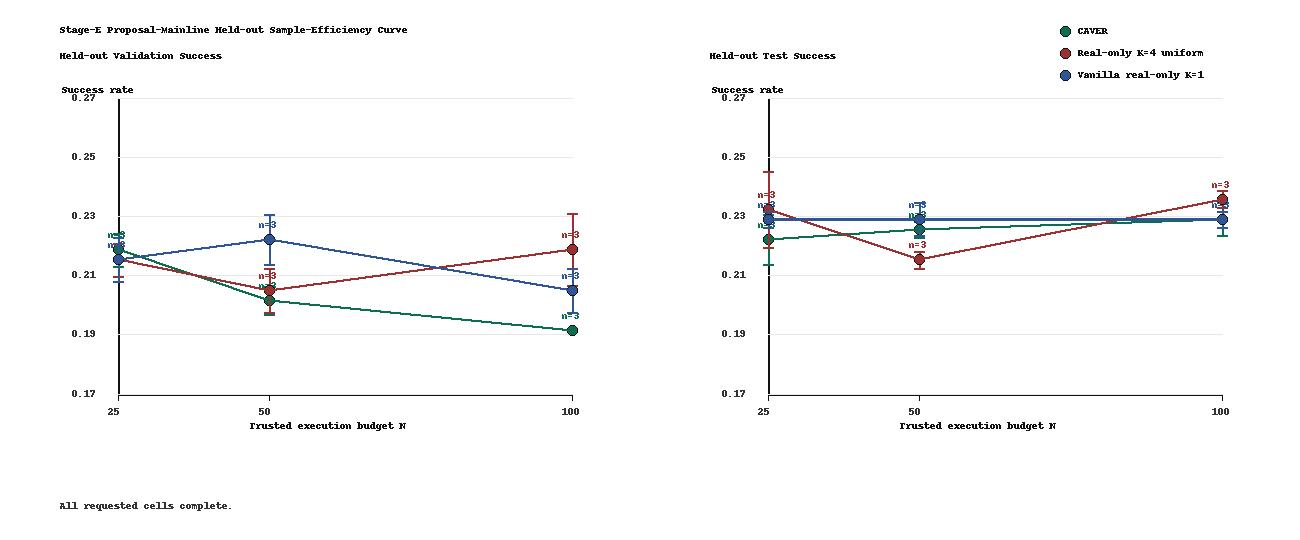
\includegraphics[width=0.92\linewidth]{figures/stagee_heldout_budget_curve_with_k1.pdf}
\caption{Strict Stage-0 held-out checkpoint curve for $N\in\{25,50,100\}$. Strict CAVER mainly supports backend-data efficiency, while vanilla $K=1$ remains a strong raw-success baseline. \label{fig:stage0_budget_curve_results}}
\end{figure}

Three caveats are intentionally left visible. First, the strict CAVER curve supports an admitted-update-data efficiency claim, not a stronger claim that CAVER needs fewer trusted executions to reach a higher success rate. Second, vanilla $K=1$ is a strong baseline in this simulation setting and must remain in the main comparison. Third, strict CAVER's conservative gate admits a small subset of successful executions, and the admitted updates are not uniformly distributed across all five proxy families. That concentration motivates CAVER+FASR rather than being hidden.

The completed $N=50$ attribution ablations clarify why the main empirical variant moved from strict CAVER to CAVER+FASR. Table~\ref{tab:stage0_attribution_results} shows that selection-only matches strict CAVER on held-out test but uses trusted-execution-only-scale backend data; admission-only matches the uniform selector baseline but its admitted-data accounting was not retained in the current summary; no-provider remains close to strict CAVER; and no-DR is hard to interpret because two seeds admit no data and therefore skip the backend update. Success-only admission improves raw held-out test by admitting every executed success instead of applying the full LCB gate. A capped hard-family rescue variant keeps the guarded selector, writes full traces for all executed contexts, and admits a small number of hard-family near-miss failures when a family has too few successes. That variant improves $N=50$ held-out test to $0.237\pm0.007$, but increasing the rescue quota to three near misses per hard family drops held-out test to $0.223\pm0.007$ and increases backend data.

CAVER+FASR changes the rescue rule from ``admit full failed traces from hard families'' to ``preserve executed successes and add only short verified-progress repair segments.'' The resulting budget points are:
\[
\begin{array}{c|ccc}
N & 10 & 25 & 50\\
\hline
\text{held-out validation} & 0.207\pm0.003 & 0.220\pm0.008 & 0.220\pm0.005\\
\text{held-out test} & 0.233\pm0.005 & 0.237\pm0.007 & 0.240\pm0.005\\
\text{demo items} & 399 & 796 & 785\\
\text{primitive steps} & 1584 & 3149 & 3110
\end{array}
\]
These are means with standard errors over seeds $\{7,13,29\}$. The $N=25$ point is important because it directly addresses the vanilla $K=1$ pressure point: CAVER+FASR reaches held-out test $0.237$ versus $0.227$ for vanilla $K=1$, while admitting $796$ rather than $1885$ demo items. The $N=25$ and $N=50$ FASR points are independent sweeps, not one cumulative run extended from 25 to 50 contexts; this is why the mean admitted demo count can be slightly lower at $N=50$ after repair capping and seed variation. This is cleaner than full-trace hard-family rescue because it does not relabel whole failed episodes as positive imitation targets. The caveats are that the raw-success margin is modest and the $N=10$ point is a very-low-budget diagnostic rather than a complete five-family budget point.

Two fairness controls are especially important for interpreting FASR. The completed vanilla $K=1$+FASR control at $N=25$ reaches held-out test $0.223\pm0.003$, below both vanilla $K=1$ ($0.227\pm0.003$) and CAVER+FASR ($0.237\pm0.007$). Thus the current CAVER+FASR improvement is not explained by simply adding progress-label repair to a single sampled chunk. The remaining direct control is uniform $K=4$+FASR: it uses the same four-candidate wrapper and the same FASR admission/repair rule, but removes provider-aware CAVER selection. The first uniform $K=4$+FASR jobs reached held-out evaluation but failed during final RDSS compact-artifact copy-back, so their parsed log numbers are treated only as triage. Clean recovery jobs are running under the metadata-free copy-back path, and final tables should be refreshed after their \texttt{posttrain\_holdout\_summary.json} files are available.

\begin{table}[H]
\centering
\small
\caption{Stage-0 $N=50$ attribution ablations on the five LIBERO proxy families. Values are mean $\pm$ standard error over seeds $\{7,13,29\}$ unless otherwise noted. Demo items and primitive steps are the mean admitted backend data retained in the current summaries. \label{tab:stage0_attribution_results}}
\begin{tabular}{@{}lcccc@{}}
\toprule
Method & Held-out val & Held-out test & Demo items & Primitive steps \\
\midrule
Strict CAVER & $0.200 \pm 0.005$ & $0.223 \pm 0.003$ & $338$ & $1338$ \\
Uniform $K=4$ & $0.203 \pm 0.007$ & $0.213 \pm 0.003$ & $3807$ & $15194$ \\
Vanilla $K=1$ & $0.220 \pm 0.008$ & $0.227 \pm 0.005$ & $3816$ & $15238$ \\
Selection-only & $0.230 \pm 0.008$ & $0.223 \pm 0.003$ & $3793$ & $15139$ \\
Admission-only & $0.207 \pm 0.007$ & $0.213 \pm 0.005$ & -- & -- \\
Success-only admission & $0.213 \pm 0.003$ & $0.233 \pm 0.003$ & $769$ & $3049$ \\
Hard-family rescue & $0.220 \pm 0.005$ & $0.237 \pm 0.007$ & $1414$ & $5631$ \\
Hard-family rescue quota-3 & $0.203 \pm 0.009$ & $0.223 \pm 0.007$ & $1714$ & $6831$ \\
Failure-diagnostic success & $0.203 \pm 0.003$ & $0.230 \pm 0.000$ & $814$ & $3231$ \\
CAVER+FASR & $0.220 \pm 0.005$ & $0.240 \pm 0.005$ & $785$ & $3110$ \\
No-DR & $0.217 \pm 0.005$ & $0.227 \pm 0.003$ & $29^\dagger$ & $114^\dagger$ \\
No-provider & $0.210 \pm 0.005$ & $0.220 \pm 0.005$ & $662$ & $2614$ \\
\bottomrule
\end{tabular}
\vspace{0.4em}
\caption*{\footnotesize $^\dagger$No-DR admitted data for only one seed; the other two seeds skipped backend update because no trajectories were admitted. The quota-3 rescue row is a negative sweep. The CAVER+FASR row preserves successes and admits only short verified-progress repair segments, not whole failed traces.}
\end{table}

\begin{figure}[t]
\centering
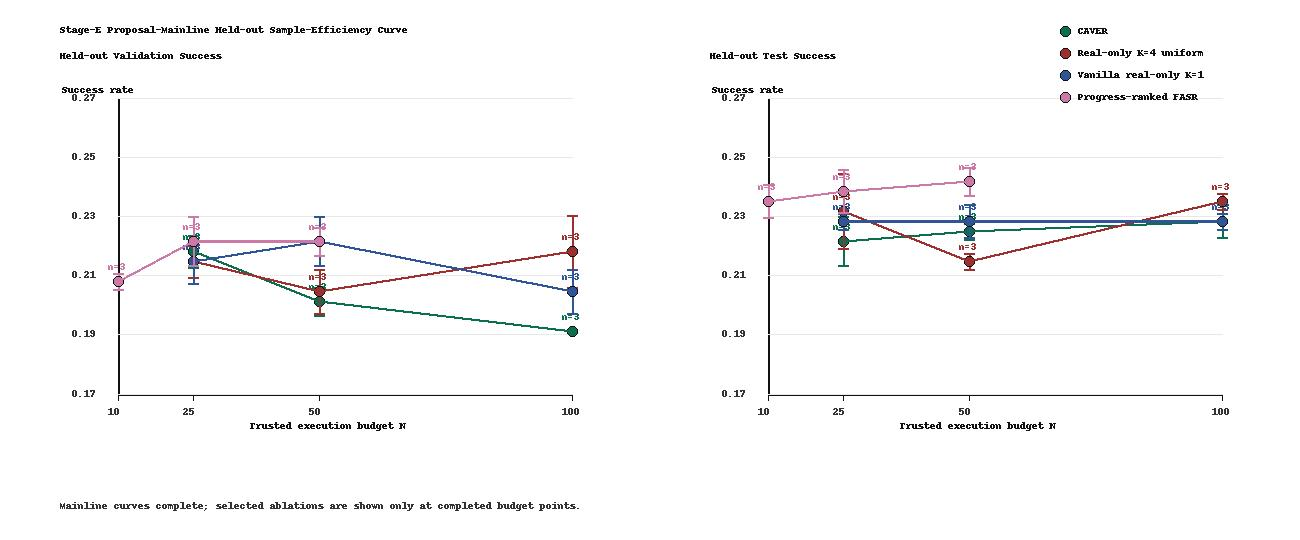
\includegraphics[width=0.92\linewidth]{figures/stagee_fasr_verified_progress_budget_curve_with_k1.pdf}
\caption{Stage-0 held-out checkpoint curves including CAVER+FASR. CAVER+FASR modestly improves mean held-out test success over vanilla $K=1$ at $N=25$ and $N=50$ while admitting fewer backend records. Missing cells reflect the different completed budget grids. \label{fig:stage0_fasr_budget_curve}}
\end{figure}

\paragraph{Shared seed real set.}
Before the matched-budget Stage-1 study, collect one common warm-start dataset of \textbf{120} PiPER decision contexts total, balanced as 40 contexts for each of the three physical Stage-1 tasks (block-to-tray, can-to-bowl, and stack). The seed set is collected with the initial $\pi_{0.5}$ backbone and a uniform random selector. Its allowed use is locked:
\begin{itemize}
    \item \textbf{All methods:} run one identical seed warm-start pass of the unchanged StepNFT backend on the executed seed trajectories, using exactly 500 gradient steps with the pinned optimizer from Step~7, producing the common starting checkpoint $\pi_{\theta_1}$ used by CAVER, real-only $\pi$-StepNFT, WoVR, and the seed-only anchor baseline.
    \item \textbf{CAVER only:} additionally fit the frozen proxy head $V_{\omega}$ and the initial calibrator $f_{\psi_0}$ on the same seed tuples.
    \item \textbf{WoVR only:} the same seed tuples may also initialize any observation normalizers or reward-scale statistics required by the public RLinf implementation, but may not be supplemented by extra real data.
\end{itemize}
No method may collect extra real interactions before the matched-budget curve starts. The shared seed set is therefore a \emph{common warm-start cost}, reported separately from the matched-budget training curves rather than silently folded into them.

\subsection{Stage-F readiness gate before the full PiPER study}
The PiPER path is treated as a gated transfer, not as completed evidence. Stage F means the hardware-readiness gate before budgeted PiPER learning. Before any budgeted hardware learning run, Stage F must pass: (i) shadow-mode execution in which the robot-control machine captures observations, forms candidates, computes safety masks and propensities, and logs the chosen action without executing learned motion; (ii) local safety-shield validation on scripted safe chunks and deliberately invalid chunks; (iii) marker/geometric end-state labeler validation against manual inspection; (iv) progress-label validation for every task on which CAVER+FASR would be used; and (v) latency logging for policy sampling, GE-Sim/provider inference, selector/calibrator scoring, and robot idle time. If the progress labels fail validation, the PiPER pilot uses strict CAVER as the fallback primary variant.

The progress-label gate is deliberately numeric. Before FASR is enabled on a PiPER task, collect at least 10 scripted or teleoperated calibration traces for that task with object-marker poses, automatic progress scores, final success labels, and manual prefix audits. The task passes only if the automatic final success label agrees with manual inspection on at least 90\% of traces, the automatic FASR prefix-eligibility decision agrees with manual inspection on at least 90\% of audited traces, and the false-eligible repair rate is at most 5\%. If marker confidence falls below 0.90 in more than 3 of the final 10 frames or the prefix audit is ambiguous, that trace is marked audit-required and cannot be used to enable FASR.

The first hardware pilot is one task and one seed only, with $N=25$, and is used to validate the loop rather than to claim significance. The full three-task study below begins only after this readiness gate passes.

\subsection{Stage 1: planned three-task PiPER study}
The real study uses exactly three tasks: block-to-tray, can-to-bowl, and two-block stack. Each Stage-1 training run is task-specific, each episode permits at most four decision contexts, and each round contains exactly $B_{\mathrm{round}}=25$ counted training contexts. Therefore the main \emph{training} budget curve $N\in\{25,50,100,200\}$ corresponds to exactly $R=N/25\in\{1,2,4,8\}$ rounds per task and per method, together with one mandatory $N=0$ seed-only anchor point that corresponds to the common seed-warmed checkpoint $\pi_{\theta_1}$ before any Stage-1 training. For the three main trainable methods (CAVER, real-only $\pi$-StepNFT, and WoVR), the study records two independent full training runs at every budget and a third independent run at $N=100$ as the primary stability point.

\paragraph{Budget accounting rule.}
Only on-policy executed decision contexts collected during Stage-1 training count toward $N$. The shared 120-context seed set does not count toward $N$. Validation and test episodes also do \emph{not} count toward $N$ and are reported separately under ``evaluation interactions.'' Every results table and success curve therefore reports two x-axes: the matched \emph{training budget} $N$ and the corresponding \emph{total real interaction count}
\[
N_{\mathrm{total}} = 120 + N + N_{\mathrm{val}}^{\mathrm{ctx}} + N_{\mathrm{test}}^{\mathrm{ctx}},
\]
where 120 is the common seed warm-start cost and $N_{\mathrm{val}}^{\mathrm{ctx}},N_{\mathrm{test}}^{\mathrm{ctx}}$ are the realized numbers of executed decision contexts consumed by validation and test episodes. The mandatory seed-size sweep repeats the same accounting for each $N_{\mathrm{seed}}\in\{0,40,80,120\}$ so readers can distinguish warm-start dependence from true Stage-1 sample efficiency.

\paragraph{Held-out evaluation.}
Every compared checkpoint is selected by the same rule: best mean success on 10 validation episodes per task drawn from a fixed held-out template list. Final reported success is mean success on 30 held-out real episodes per task drawn from a second disjoint template list shared across methods and runs, with a nonparametric bootstrap confidence interval over episodes.

\paragraph{Repeated-run and paired statistical plan.}
The final paper will report both across-run and within-run uncertainty. For each method, task, and budget, aggregate the two independent training runs (three at $N=100$) with a hierarchical bootstrap that first resamples runs and then resamples episodes within each run. In addition, the headline $N=100$ comparison uses a paired permutation test over the 30 shared held-out test templates for CAVER versus the real-only baseline and for CAVER versus WoVR. The $N=0$ seed-only anchor is always shown on the same plots so readers can see how much of any gain comes from Stage-1 training rather than from the common 120-context warm-start alone.


\paragraph{Matched-budget world-model baseline.}
The WoVR/RLinf baseline receives the same common seed-warmed starting checkpoint $\pi_{\theta_1}$, the same shared 120-context seed set, and the same real training budget $N$ as CAVER. In addition, it may use imagined rollouts generated by its own world-model stack, but its real interaction count may never exceed the current budget point $N$. The imagined-rollout multiplier is fixed before Stage 1 at $M=32$ imagined candidate rollouts per verified context and is not re-tuned online. The entire baseline is pinned by one immutable local RLinf config file \texttt{configs/wovr\_piper\_h4.yaml}, stored with a SHA256 checksum in \texttt{manifest.lock}. That config is derived once from the locked RLinf WoVR-LIBERO release and changes only the study-specific fields: policy initialization path $\pi_{\theta_1}$, PiPER environment wrapper, chunk horizon $H=4$, real-budget cap $N$, rollout horizon 4 chunks, imagined multiplier $M=32$, one policy-update block after each 25-context round, and exactly 500 optimizer steps per update block. All other RLinf/WoVR fields remain the upstream defaults at the locked commit and may not be changed between methods, budgets, or seeds except for the random seed itself. If the public RLinf/WoVR stack requires more real data than the matched budget to become operational on PiPER, the comparison is reported as ``not feasible under the matched-budget protocol'' rather than silently given extra real data.

\subsection{Baselines and ablations}
\paragraph{Primary baselines.}
\begin{itemize}
    \item \textbf{Seed-only anchor:} the common seed-warmed checkpoint $\pi_{\theta_1}$ with no Stage-1 training. This baseline isolates the contribution of the shared 120-context warm-start.
    \item \textbf{Real-only baseline:} $\pi$-StepNFT on $\pi_{0.5}$ using the same candidate-generation wrapper but a uniform selector over the $K$ candidates, with every executed trajectory admitted to training and no selective-verification correction.
    \item \textbf{Vanilla real-only $K=1$:} the stricter single-candidate real-only baseline for Stage 1. This baseline removes the shared $K=4$ candidate wrapper and tests whether CAVER improves over ordinary executed-trajectory fine-tuning rather than only over a matched uniform-candidate wrapper.
    \item \textbf{World-model-heavy baseline:} WoVR through RLinf, using imagined rollouts as the primary update signal \citep{jiang2026wovr,rlinfrepo2026}.
\end{itemize}

\paragraph{Mandatory attribution ablations.}
\begin{itemize}
    \item \textbf{Strict CAVER:} keep CAVER's selector, exact-propensity logging, DR calibrator, and LCB admission rule, but remove FASR repair segments. This is the conservative base rule.
    \item \textbf{Selection-only:} keep CAVER's selector and exact-propensity logging, but admit every executed trajectory to StepNFT with no conservative admit/abstain gate.
    \item \textbf{Admission-only:} use the same uniform safe-set selector as the real-only baseline, but apply CAVER's DR calibrator and conservative admit/abstain rule before StepNFT.
    \item \textbf{Random verification:} keep the same conservative gate as full CAVER, but choose the executed safe candidate uniformly at random.
    \item \textbf{Value-only verification:} pick the candidate with the highest raw proxy value and remove uncertainty/diversity/novelty terms from the selector score.
    \item \textbf{No-DR ablation:} keep the selector and admission rule, but replace DR pseudo-outcomes with direct executed-data supervision only.
\end{itemize}

\paragraph{Mandatory sensitivity analyses.}
\begin{itemize}
    \item \textbf{Seed-size curve:} rerun the main $N\in\{0,25,50,100\}$ study with shared seed sizes $N_{\mathrm{seed}}\in\{0,40,80,120\}$ total decision contexts, always reporting both against $N$ and against $N_{\mathrm{total}}$.
    \item \textbf{Frozen-vs-refreshed utility head:} compare the main frozen $V_{\omega}$ against a lightweight refreshed variant that refits $V_{\omega}$ every two rounds on cumulative executed tuples while keeping GE-Sim frozen and keeping selector coefficients fixed.
    \item \textbf{Proxy-target sensitivity:} replace the main $u^{\mathrm{proxy}}=0.5\,s^{\mathrm{bin}}+0.5\,q^{\mathrm{prog}}$ target with $u^{\mathrm{proxy}}_{\alpha}=\alpha s^{\mathrm{bin}}+(1-\alpha)q^{\mathrm{prog}}$ for $\alpha\in\{0.25,0.5,0.75,1.0\}$.
    \item \textbf{No-provider ablation:} keep the same executed-only backend and selector budget, but remove GE-Sim and use only raw backbone/context features for verification.
    \item \textbf{Weighted-update secondary ablation:} keep the same admitted executed set, but multiply each StepNFT pair by $\max\{0,\LCB_r(z_{r,c,A_{r,c}})-\tau\}$ before the otherwise unchanged StepNFT loss. This remains secondary and is not part of the main comparison claim.
\end{itemize}

\paragraph{Fairness rule.}
All methods share the same public $\pi_{0.5}$ base checkpoint, the same local \texttt{pi05\_piper\_h4} policy interface, the same seed real dataset, the same common seed-warm-start checkpoint $\pi_{\theta_1}$, the same deterministic safety shield, the same Stage-0 proxy families, the same Stage-1 tasks, the same Stage-1 real-rollout budget, and the same final evaluation protocol. CAVER+FASR and the real-only baseline also share the same candidate-generation wrapper and the same executed-update backend: the same $K=4$ candidate draws per decision context, the same chunk horizon $H=4$, the same LoRA target modules, the same optimizer, the same learning-rate schedule, the same batch size, the same positive--negative pair construction, the same gradient clip, and the same number of update steps. The real-only baseline uses a uniform selector and admits every executed trajectory to the StepNFT trainer; CAVER+FASR differs by using provider-based scoring, exact-propensity logging, doubly robust calibration, conservative admission, and verified-progress repair segments before examples enter that same trainer. The mandatory strict-CAVER, selection-only, admission-only, and no-DR ablations are included precisely so that any observed gain can be attributed more cleanly to verification allocation, conservative admission, failure-aware repair, or their combination rather than to the unchanged StepNFT backend itself.

\subsection{Metrics}
The current Stage-0 report and planned Stage-1 study use overlapping but not identical metrics. Stage 0 reports simulated held-out validation/test success, admitted backend data, and ablations. Stage 1 will add real-robot success, real interaction accounting, latency, and hardware safety diagnostics. The main metrics are:
\begin{itemize}
    \item \textbf{Held-out real-robot success rate:} mean binary success over the 30 final test episodes per task.
    \item \textbf{Success gain per 100 verified contexts:}
    \[
    G_{100}=100\,\frac{S(200)-S(25)}{200-25},
    \]
    where $S(N)$ is the held-out success rate after training with budget $N$.
    \item \textbf{Stage-0 selector regret:}
    \[
    \mathrm{Regret}_{\mathrm{S0}}=\frac{1}{C}\sum_{c=1}^{C}\Big(\max_{k\le K}u^{\mathrm{proxy}}_{c,k}-u^{\mathrm{proxy}}_{c,A_c}\Big)
    \]
    on matched-start simulation contexts with fully known proxy labels.
    \item \textbf{Cross-method calibration metrics:} to make Brier/ECE comparable for CAVER, real-only $\pi$-StepNFT, and WoVR, fit one \emph{common post-hoc diagnostic predictor} $g_{\mathrm{eval}}$ separately for each method using only that method's executed training data and the same method-agnostic executed feature vector
    \[
    z^{\mathrm{exec}}_{r,c}=[e_{r,c},\phi_a(a_{r,c,A_{r,c}}),\text{task one-hot}],
    \qquad
    g_{\mathrm{eval}}(z)=\sigma(h_{\chi}(z)),
    \]
    where $h_{\chi}$ is a 2-layer width-256 GELU MLP and $\sigma$ is the sigmoid output link. The predictor is trained with binary cross-entropy
    \[
    L_{\mathrm{eval}}(\chi)=
    -\sum_i\Big(Y_i\log g_{\mathrm{eval}}(z_i)+(1-Y_i)\log(1-g_{\mathrm{eval}}(z_i))\Big)
    \]
    using AdamW with learning rate $10^{-3}$, betas $(0.9,0.999)$, weight decay $10^{-4}$, batch size 128, maximum 50 epochs, early stopping patience 5 on fold-validation BCE, and 5-fold cross-fitting. Brier and 10-bin equal-frequency ECE are computed from the resulting out-of-fold probabilities $g_{\mathrm{eval}}(z)$ on validation/test episodes. This is a \emph{common downstream diagnostic}, not each method's native online confidence model. Whenever the paper says ``better calibration'' in a cross-method table, it refers to this common post-hoc predictor unless the text explicitly says ``online CAVER calibrator.'' The online CAVER calibrator $\bar\mu_r(z)$ is reported separately as an internal diagnostic.
    \item \textbf{Interaction efficiency:} wall-clock time and real training interactions required to reach the target success threshold $S^\star=0.70$ on each task.
    \item \textbf{Deployment latency:} median and 95th-percentile wall-clock latency per decision context, broken into policy sampling, provider rollout/inference, selector/calibrator scoring, and robot idle time waiting for the verification decision.
    \item \textbf{Budget transparency:} every success plot is reported twice, once against matched training budget $N$ and once against total real interaction count $N_{\mathrm{total}}$, and both plots include the seed-only point at $N=0$.
\end{itemize}
The continuous progress score $\bar Y$ is reported only as a diagnostic.

\subsection{What the current Stage-0 result supports}
The current Stage-0 result is strong enough to justify PiPER integration and a gated real-robot pilot, but it should still be read carefully. Strict CAVER supports a backend-data-efficiency story: it preserves comparable held-out performance while materially reducing the amount of trusted executed data consumed by the unchanged backend. CAVER+FASR is now the stronger Stage-0 empirical variant: it reaches held-out test $0.237$ at $N=25$ and $0.240$ at $N=50$, while using far less backend data than vanilla $K=1$. The completed vanilla $K=1$+FASR control at $N=25$ reaches only $0.223$, which is evidence that CAVER+FASR is not just FASR attached to the vanilla baseline. However, the raw-success margin is still modest, the $N=10$ point is diagnostic rather than full-family, the uniform $K=4$+FASR control is still awaiting clean recovery summaries, and none of the Stage-0 results prove completed real-robot sample efficiency.

This matters for how the next stage should be judged. Stage 1 should test whether the same backend-data efficiency pattern survives transfer to PiPER and whether CAVER+FASR becomes real-interaction efficiency under hardware constraints. The necessary real-robot claim is stronger than the current Stage-0 claim: CAVER+FASR should either outperform real-only at a matched $N$, reach comparable success at a smaller $N$, or provide a clear systems benefit by matching success with substantially less admitted update data. If Stage 1 reproduces only the third pattern, the combined paper should remain a selective-admission/data-efficiency paper rather than a raw-success paper.

The Stage-0 ablations also motivate a conservative implementation decision before the full hardware study. We should not delay PiPER readiness work for another broad redesign, because camera calibration, safety filtering, labeler validation, latency measurement, and shadow-mode logging do not spend matched training budget and are needed regardless of the final admission rule. However, the simulation section should be refreshed once uniform $K=4$+FASR finishes, because that control is the cleanest way to separate provider-aware selection from progress-label repair. We should also \emph{not} launch the full three-task PiPER study before the progress-label assumption behind FASR is validated on hardware. The first hardware pilot should include (i) CAVER+FASR as the primary candidate, (ii) strict CAVER as the fallback/base rule, and (iii) the real-only $K=4$ and vanilla $K=1$ baselines as feasible. Shadow-mode logs should specifically inspect $\mu$, $\sigma$, LCB, admitted-positive rate, hard-family coverage, skipped-update frequency, verified-progress repair counts, progress-label agreement, and provider latency. If progress labels are unreliable, fall back to strict CAVER or a threshold-relaxed admission rule for the full Stage-1 curve.

\section{Concrete implementation plan: Stage-0 LIBERO and Stage-1 PiPER instantiations}
This section pins two concrete instantiations of the abstract CAVER interfaces from the main method. Stage 0 is the simulation proxy study: LIBERO acts as the trusted execution environment, a LIBERO-specific execution adapter instantiates $\Gamma_{\mathrm{exec}}$, a LIBERO-to-GE-Sim bridge instantiates $\Phi_{\Omega}$, and the simulator task-success signal instantiates $M_{\mathrm{task}}$. Stage 1 is the real transfer study: the concrete execution adapter is denoted
\[
\Gamma_{\pi\rightarrow p}\coloneqq \Gamma_{\mathrm{exec}},
\]
and maps raw $\pi_{0.5}$ chunks into PiPER joint/gripper execution commands. The concrete provider adapter is denoted
\[
\Phi_{\mathrm{GE}}\coloneqq \Phi_{\Omega},
\]
and maps those execution commands into the public GE-Sim conditioning format. The concrete safety shield is the PiPER URDF-based hard filter described below, and the concrete verified labeler is the marker-based geometric checker used in the Stage-1 real study. Porting CAVER to another robot changes these implementation modules and the associated local configs, but it does \emph{not} change selector scoring, exact propensity logging, doubly robust correction, calibrator fitting, or the StepNFT-style executed-update backend.

\begin{table}[H]
\centering
\small
\caption{Boundary between completed Stage-0 evidence and planned Stage-1 hardware evidence.\label{tab:stage0_stage1_boundary}}
\begin{tabularx}{\linewidth}{@{}p{3.2cm}XX@{}}
\toprule
Component & Completed Stage 0 & Planned Stage 1 \\
\midrule
Trusted execution environment & LIBERO simulation. & PiPER hardware. \\
Execution adapter & LIBERO action adapter with finite, shape, and magnitude checks. & PiPER joint/gripper adapter with URDF and workspace checks. \\
Provider adapter & LIBERO-to-GE-Sim compatibility bridge. & PiPER-to-GE-Sim compatibility bridge. \\
Verified labeler & Simulator task-success signal plus progress diagnostics. & Marker-based geometric task labeler with audit triggers. \\
Backend validated so far & Exact offline rollout-batch export for admitted successful records. & Full mirrored-pair StepNFT backend pinned in Step 7. \\
Claim supported now & CAVER+FASR gives simulation selective-admission/sample-efficiency evidence; strict CAVER is the conservative base ablation. & Real-robot sample efficiency remains to be tested. \\
\bottomrule
\end{tabularx}
\end{table}

\subsection{Concrete Stage-0 LIBERO simulation instantiation}
Stage 0 is not just a debugging convenience; it is the concrete simulation instantiation used to fit the proxy head, lock selector defaults, and validate the roundwise protocol before any PiPER run is attempted. Each Stage-0 run uses LIBERO as the trusted execution environment, keeps the same chunk horizon $H=4$, candidate count $K=4$, round size $B_{\mathrm{round}}=25$, and matched counted-context budgets used later, and compares CAVER directly against the trusted-execution-only $\pi$-StepNFT path plus attribution ablations on five LIBERO proxy families.

The Stage-0 bridge preserves the method-level interfaces rather than introducing a separate algorithm. Raw $\pi_{0.5}$ chunks are converted into LIBERO simulator control commands through a deterministic execution adapter, invalid candidate tensors are rejected by finite/shape/magnitude checks before selection, the same chunks are mapped into GE-Sim-compatible provider arrays through a LIBERO-to-GE-Sim compatibility map, and the trusted label comes from the simulator's task-completion signal together with the fixed Stage-0 progress diagnostics. This makes the Stage-0 study a concrete provider-aware selective-verification experiment in its own right, not a placeholder for the PiPER section.

\subsection{Two-machine deployment}
Use two machines throughout the project.
\begin{itemize}
    \item \textbf{Robot-control machine (Ubuntu 20.04 + ROS Noetic).} Runs \texttt{piper\_sdk}, \texttt{piper\_ros}, camera drivers, the execution bridge, and the reset/checklist UI.
    \item \textbf{Learning machine (Ubuntu 22.04 + GPU).} Runs \texttt{openpi}, Genie Envisioner / GE-Sim inference, Stage-0 LIBERO experiments, the DR calibrator, the selector, the replay buffer, and the baseline training code.
\end{itemize}
This split matches the public software assumptions: openpi documents a \texttt{uv} workflow on Ubuntu 22.04, RLinf recommends Docker on Ubuntu 22.04, and the PiPER ROS stack targets ROS Noetic on Ubuntu 20.04 \citep{openpi2026repo,rlinfrepo2026,agilex2026piperros}.

\subsection{Pinned backbone config and software revisions}

The proposal now pins the concrete software stack closely enough that the action semantics and baseline interfaces are no longer branch-dependent.

\begin{table}[H]
\centering
\small
\caption*{Pinned public revisions and local config names}
\begin{tabularx}{\linewidth}{@{}p{3.4cm}X@{}}
\toprule
Artifact & Locked identifier used in this study \\
\midrule
openpi repository & commit \texttt{fdc03f527881cdfc8ae1a168ed6a20c60edbbbcc} \\
Backbone weights & \texttt{gs://openpi-assets/checkpoints/pi05\_base/params} \\
Local policy config & \texttt{pi05\_piper\_h4} = public \texttt{pi05\_libero} config with action horizon changed to $H=4$ and outputs changed to \texttt{PiperJointDeltaOutputs} \\
Genie Envisioner / GE-Sim & commit \texttt{0e0de7e2ed8ea04e6ba41d47c93964ae65e5fbd2} \\
pi-StepNFT backend & commit \texttt{140eece2ef7e8574c34c69a221fd4e3f56c2423c} \\
RLinf / WoVR baseline & commit \texttt{e62de7767f41a61d58eb15d916e8809c70610672} and Docker tag \texttt{rlinf/rlinf:agentic-rlinf0.2-maniskill\_libero} \\
Local WoVR config & \texttt{configs/wovr\_piper\_h4.yaml}: policy init $=\pi_{\theta_1}$, PiPER env wrapper, horizon $H=4$, rollout horizon 4 chunks, imagined multiplier $M=32$, one update block per 25-context round, 500 optimizer steps per block; SHA256 stored in \texttt{manifest.lock} \\
PiPER ROS stack & \texttt{piper\_ros} \texttt{noetic} branch; exact URDF checksum stored in \texttt{manifest.lock} before the first real run \\
\bottomrule
\end{tabularx}
\end{table}

If any public repository changes after these revisions, the study still stays on the locked identifiers above. Before the first real run, the codebase must materialize a \texttt{manifest.lock} file containing these exact SHAs, the GE-Sim weight identifier, the PiPER URDF checksum, the SHA256 checksums of the two local config files \texttt{pi05\_piper\_h4.py} and \texttt{wovr\_piper\_h4.yaml}, and the local repository commit.

\subsection{Verified setup commands}
\textbf{Backbone and general training stack.}
\begin{lstlisting}
mkdir -p robot_posttrain_ws/third_party
cd robot_posttrain_ws/third_party

git clone --recurse-submodules \
  https://github.com/Physical-Intelligence/openpi.git
cd openpi
GIT_LFS_SKIP_SMUDGE=1 uv sync
GIT_LFS_SKIP_SMUDGE=1 uv pip install -e .
\end{lstlisting}
These commands follow the public openpi setup path \citep{openpi2026repo}. After installation, add the local config \texttt{pi05\_piper\_h4} by copying the public \texttt{pi05\_libero} config and changing only the action horizon to 4 and the output adapter to \texttt{PiperJointDeltaOutputs}; the weight loader remains the public \texttt{pi05\_base} checkpoint.

\textbf{Frozen provider (Genie Envisioner / GE-Sim).}
\begin{lstlisting}
cd /path/to/robot_posttrain_ws/third_party
git clone https://github.com/AgibotTech/Genie-Envisioner.git
conda create -n genie_envisioner python=3.10.4
conda activate genie_envisioner
cd Genie-Envisioner
pip install -r requirements.txt
# Download GE-Sim weights and required Cosmos2 components
# then run the released inference example on local image/action files.
python gesim_video_gen_examples/infer_gesim.py \
  --config_file=configs/cosmos_model/acwm_cosmos.yaml \
  --image_root=gesim_video_gen_examples/sample_0 \
  --extrinsic_root=gesim_video_gen_examples/sample_0 \
  --intrinsic_root=gesim_video_gen_examples/sample_0 \
  --action_path=gesim_video_gen_examples/sample_0/actions.npy \
  --output_path=gesim_video_gen_examples/sample_0_res
\end{lstlisting}
These commands match the public GE-Sim inference path released in the repository README \citep{genierepo2026}.

\textbf{PiPER robot stack.}
\begin{lstlisting}
cd /path/to/robot_posttrain_ws/third_party
git clone https://github.com/agilexrobotics/piper_sdk.git
git clone https://github.com/agilexrobotics/piper_ros.git

cd piper_sdk
pip3 install python-can
pip3 install .

cd ../piper_ros
git checkout noetic
source /opt/ros/noetic/setup.bash
catkin_make
bash find_all_can_port.sh
bash can_activate.sh can_piper 1000000 "<USB_PORT>"
\end{lstlisting}
These steps are taken directly from the public PiPER SDK and PiPER ROS instructions \citep{agilex2026pipersdk,agilex2026piperros}.

\textbf{Camera calibration.}
Use three fixed RGB cameras rigidly mounted relative to the table and label them \texttt{head}, \texttt{hand\_left}, and \texttt{hand\_right} to match the GE-Sim config convention. Calibrate intrinsics for each camera with the vendor's checkerboard routine. Calibrate each base-to-camera transform once with a standard hand-eye or checkerboard-in-base-frame routine; if the AgileX hand-eye package is convenient on the installed stack, use that path \citep{agilex2026handeye}. Store the resulting matrices in \texttt{configs/camera/piper\_multiview.yaml}. Because all cameras are static, the same extrinsics are reused across all frames of an episode.

\textbf{LIBERO Stage 0.}
\begin{lstlisting}
conda create -n libero python=3.8.13
conda activate libero
cd /path/to/robot_posttrain_ws/third_party
git clone https://github.com/Lifelong-Robot-Learning/LIBERO.git
cd LIBERO
pip install -r requirements.txt
pip install -e .
python benchmark_scripts/download_libero_datasets.py \
  --datasets libero_object --use-huggingface
\end{lstlisting}
This follows the public LIBERO repository and dataset instructions \citep{libero2023benchmark,liberorepo2026}.

\textbf{Stage-0 simulation protocol.}
The concrete Stage-0 study uses the LIBERO adapter above to run the same candidate/chunk protocol that will later be used on PiPER: sample $K=4$ chunks from $\pi_{0.5}$, score them with the frozen provider and the fixed proxy-plus-calibrator stack, execute at most one safety-approved chunk per counted context, log the exact propensity, and train the unchanged StepNFT-style backend only on admitted executed trajectories or verified-progress repair segments. Stage-0 headline plots compare CAVER+FASR against both the matched trusted-execution-only $K=4$ baseline and the stricter vanilla $K=1$ baseline under matched counted-context budgets on the five LIBERO proxy task families before any Stage-1 transfer claim is made. The completed strict-CAVER held-out $N\in\{25,50,100\}$ curve supports matched-budget admitted-update-data efficiency as the conservative base result. CAVER+FASR adds $N\in\{10,25,50\}$ evidence and shows a modest raw held-out-test improvement over vanilla $K=1$ at $N=25$ and $N=50$ with far less admitted backend data. It still does not prove the stronger real-robot claim that CAVER needs fewer trusted executions on hardware.

\textbf{World-model-heavy baseline (WoVR through RLinf).}
\begin{lstlisting}
cd /path/to/robot_posttrain_ws/third_party
git clone https://github.com/RLinf/RLinf.git
# Follow the Docker-first installation path recommended by RLinf.
docker pull rlinf/rlinf:agentic-rlinf0.2-maniskill_libero
\end{lstlisting}
RLinf explicitly recommends Docker for embodied RL and explicitly advertises official support for world-model-based VLA RL fine-tuning with WoVR \citep{rlinfrepo2026}.

\textbf{Real-only baseline backend.}
\begin{lstlisting}
cd /path/to/robot_posttrain_ws/third_party
git clone https://github.com/wangst0181/pi-StepNFT.git
\end{lstlisting}
The released code is the reference backend for both the real-only baseline and the CAVER update layer \citep{pistepnftrepo2026}.

\subsection{Concrete PiPER--GE-Sim data interface for the current study}
The critical concrete integration detail is how sampled policy chunks become \emph{both} PiPER execution commands and GE-Sim conditioning files in the present study. This subsection deliberately pins that interface for the current implementation; other robots would replace only this bridge while leaving the CAVER verification layer unchanged.

\paragraph{Execution-space file.}
For every candidate, write an \texttt{exec\_actions.npy} file of shape $H\times 7$ with rows
\[
[q_1,q_2,q_3,q_4,q_5,q_6,g].
\]
These are the exact absolute joint/gripper targets that will be streamed to PiPER at 10 Hz. This file is the source of truth for real execution.

\paragraph{Provider-space file.}
From the same execution chunk, deterministically construct
\[
\tilde a^{\mathrm{GE}}_{r,c,k}=\Phi_{\mathrm{GE}}(a_{r,c,k})\in\mathbb R^{H\times 16},
\]
and write it to \texttt{actions.npy} in the GE-Sim input folder. Each row has the public dual-arm pose-style layout
\[
[x,y,z,q_x,q_y,q_z,q_w,g]_{\text{left}}\ \Vert\
[x,y,z,q_x,q_y,q_z,q_w,g]_{\text{right}},
\]
where the left arm is the active PiPER arm and the right arm is a fixed parked dummy trajectory.

\paragraph{Camera files.}
For every context, write synchronized RGB frames for the three fixed views \texttt{head}, \texttt{hand\_left}, and \texttt{hand\_right}. Store one intrinsics file and one base-to-camera extrinsics file per view. Because all three cameras are static, the same extrinsics are reused across all frames of the episode; the runtime wrapper simply copies the same matrix into the provider input directory for each timestep.

\paragraph{Feature-extraction rule.}
GE-Sim predicts a sequence of $H$ future frames for every configured view. CAVER always extracts the cheap future embedding from the \emph{final predicted head-view frame} only. The left and right auxiliary views are retained to condition the provider, not to define the final feature.

\paragraph{Week-1 interface test.}
Before any learning experiment begins, run one interface sanity test on 20 replayed Stage-0 contexts:
\begin{enumerate}
    \item sample one candidate chunk from $\pi_{0.5}$,
    \item write both \texttt{exec\_actions.npy} and GE-Sim \texttt{actions.npy},
    \item verify that PiPER forward kinematics applied to \texttt{exec\_actions.npy} reproduces the left-arm pose entries written into \texttt{actions.npy}$\,$ to within $5\times10^{-3}$ m and $2^\circ$,
    \item verify that GE-Sim runs without schema errors and produces an output frame sequence of length $H$.
\end{enumerate}
If any of these checks fail by the end of week 4, the contingency provider in Appendix~\ref{app:contingency} is activated and the paper must say so explicitly.

\subsection{Frozen vs trainable modules}
\begin{table}[H]
\centering
\small
\caption*{What changes online and what never changes in Stage 1}
\begin{tabularx}{\linewidth}{@{}p{3.1cm}p{2.0cm}X@{}}
\toprule
Module & Status in Stage 1 & Exact rule \\
\midrule
$\pi_{0.5}$ vision/language encoders & Frozen & Used to build context features and start-state embeddings only. \\
GE-Sim provider $\mathcal T_{\Omega}$ & Frozen & Never fine-tuned in the mainline method. \\
Future-frame encoder $F_{\rho}^{\mathrm{frz}}$ & Frozen & Same feature space for all rounds and all methods. \\
Proxy head $V_{\omega}$ & Frozen & Trained in Stage 0 + seed data only. \\
Selector coefficients & Frozen & Tuned once on Stage 0 validation and never learned online. \\
Calibrator $f_{\psi_r}$ & Updated each round & Refit on all verified data accumulated so far. \\
Backbone action-head LoRA modules & Updated each round if enough positives exist & Modified only by the unchanged StepNFT loss on admitted executed trajectories. \\
\bottomrule
\end{tabularx}
\end{table}


\subsection{Stage-0 tuning grid and Stage-1 defaults}
Table~\ref{tab:hparams} lists the fixed hyperparameters and tuning ranges used in the implementation. If Stage-0 validation leaves multiple settings statistically indistinguishable, choose the tie-break default in the rightmost column.

\begin{table}[H]
\centering
\small
\caption{Exact tuning grid and tie-break defaults used in the implementation.\label{tab:hparams}}
\begin{tabularx}{\linewidth}{@{}p{3.7cm}p{5.1cm}X@{}}
\toprule
Component & Search / fixed value & Tie-break default used if validation is inconclusive \\
\midrule
Candidate count $K$ & Fixed at 4 & 4 \\
Chunk horizon $H$ & Fixed at 4 & 4 \\
Selector value weight $\lambda_V$ & $\{1.0,1.5,2.0\}$ & 2.0 \\
Selector uncertainty / disagreement / novelty weights $(\lambda_U,\lambda_D,\lambda_N)$ & Each in $\{0,0.25,0.5\}$ & $(0.25,0.25,0.25)$ \\
Selector temperature $T$ & $\{0.25,0.5,1.0\}$ & 0.5 \\
Exploration floor $\epsilon$ & $\{0.05,0.10,0.20\}$ & 0.10 \\
Conservative multiplier $\kappa$ & $\{0.5,1.0\}$ & 0.5 \\
Acceptance threshold $\tau$ & $\{0,0.05,0.10\}$ & 0.05 \\
Proxy head $V_\omega$ & AdamW, lr $10^{-3}$, batch 256, 30 epochs max, early-stop patience 5 & Same as search setting \\
Calibrator $f_{\psi_r}$ & AdamW, lr $3\times10^{-4}$, batch 256, 80 epochs max, early-stop patience 8 & Same as search setting \\
Retrospective DR diagnostic & 5-fold cross-fitting with the same 2-layer width-256 MLP family as $f_{\psi_r}$ & 5 folds \\
Action-head adaptation & LoRA rank 16, LoRA scale $\alpha=32$, dropout 0 & Same as search setting \\
StepNFT backend update & AdamW, lr $10^{-5}$, batch 16 positive--negative pairs, max 500 gradient steps per round, gradient clip 1.0 & Same as search setting \\
\bottomrule
\end{tabularx}
\end{table}

\subsection{Minimal logs that must exist for reproducibility}
Before the first real run, write one immutable \texttt{manifest.lock} file containing the exact openpi, GE-Sim, RLinf, and pi-StepNFT SHAs; the checkpoint path \texttt{gs://openpi-assets/checkpoints/pi05\_base/params}; the local config names \texttt{pi05\_piper\_h4} and \texttt{wovr\_piper\_h4.yaml}; the PiPER URDF checksum; the GE-Sim weight identifier; and every study random seed (policy sampling, selector sampling, StepNFT sampling, bootstrap-mask sampling, and train/val/test template shuffles). For every decision context, record run ID, round ID, episode ID, context ID, task ID, and language instruction; all three RGB observation paths, proprioception vector, and camera intrinsics/extrinsics IDs; all execution-space candidate chunks $a_{r,c,1:K}$; all provider-space arrays $\tilde a^{\mathrm{GE}}_{r,c,1:K}$; all predicted future-frame file paths from GE-Sim; all cheap features $z_{r,c,1:K}$; selector scores $s_{r,c,1:K}$ and exact propensities $p_{r,c,1:K}$; safety-mask membership $\mathcal K^{\mathrm{safe}}_{r,c}$ and any safety reason codes; executed candidate index $A_{r,c}$; binary outcome $Y_{r,c}$, optional diagnostic progress $\bar Y_{r,c}$, audit flags, safety-abort flags, and timeout/reset flags; plus model/version hashes for openpi, GE-Sim, RLinf, pi-StepNFT, the PiPER URDF, and the local repository.


\subsection{Hard safety shield implementation}
The safety shield in Step~4b is implemented on the robot-control machine and is shared unchanged by CAVER, the real-only baseline, the seed-data collection pass, and any WoVR real execution. The bridge evaluates every candidate chunk with the PiPER URDF, the calibrated table plane, and a padded collision model \emph{before} the selector is allowed to sample a real action. The exact rejection rules are the ones in Step~4b: joint bounds, velocity caps, acceleration caps, workspace-box limits, and padded self/table-collision checks. Runtime monitoring then re-checks the currently observed joint state at 20 Hz and triggers the same abort rules during execution. Every rejection or abort is logged with a categorical reason code from the fixed set
\[
\begin{aligned}
\{&\texttt{joint\_limit},\texttt{velocity},\texttt{acceleration},\texttt{workspace},\\
  &\texttt{self\_collision},\texttt{table\_collision},\texttt{heartbeat},
    \texttt{tracking},\texttt{manual\_estop}\}.
\end{aligned}
\]
The final paper will report the frequency of each reason code per method and per task so that any success gain cannot hide an unsafe execution pattern.

\subsection{Real experiment protocol}
Each real episode begins from a template object placement defined in \texttt{configs/piper\_tasks.yaml}. An episode ends when success is reached, when four decision contexts have been used, or when a hard wall-clock timeout of 60 s is reached. Between episodes, the operator performs a fixed reset procedure and checks a three-item list: object placement, camera pose, and gripper state. This reset is not part of the learning algorithm, but it is fixed across all methods to keep the budget comparison fair.

The training/evaluation accounting is also fixed:
\begin{itemize}
    \item Stage-1 training episodes contribute to the matched budget $N$ only through counted decision contexts.
    \item Validation and test episodes are logged separately and never mixed into the training buffers or the calibrator fits.
    \item Any evaluation episode that ends in \texttt{safety\_abort}, \texttt{manual\_estop}, or wall-clock timeout is scored as failure ($Y=0$) for the success metric.
    \item Human audits are permitted only for end-state labeling when the marker tracker reports low confidence; they are not allowed to modify action choices, StepNFT pair construction, or success thresholds.
\end{itemize}

\subsection{Contingency plan if GE-Sim integration fails early}
The proposal should remain executable even if the primary provider is delayed. The contingency trigger is simple: if the team cannot produce stable short-horizon GE-Sim predictions on Stage-0 LIBERO trajectories by the end of week 4, freeze the current CAVER interface and temporarily substitute the lightweight local provider described in Appendix~\ref{app:contingency}. That contingency is \emph{not} the main claim and should be clearly labeled as such in the eventual paper.

\section{Claim scope and evidence}
The current paper claim is intentionally narrow: CAVER is a selective-verification layer for flow-based VLA post-training under strict matched trusted-execution budgets, not a fundamentally new RL algorithm. The completed Stage-0 evidence supports CAVER+FASR as the main simulation variant: it modestly improves held-out test success over vanilla $K=1$ at low budgets while using much less admitted backend data, and the completed $K=1$+FASR control does not explain that improvement. Strict CAVER remains important as the conservative base rule showing admitted-update-data efficiency without repair segments. The current evidence does not yet prove broad raw-success superiority or completed real-robot sample efficiency, and the uniform $K=4$+FASR fairness control remains an active recovery run rather than a finalized table entry.

\paragraph{Limitations that remain after the current revision.}
First, all completed evidence is LIBERO simulation evidence; PiPER hardware remains a planned Stage-F/Stage-1 path. Second, the raw held-out-success margin of CAVER+FASR over vanilla $K=1$ is modest, so the strongest current story is selective admission with much lower backend data rather than broad dominance. Third, FASR depends on reliable progress labels; if those labels are noisy on hardware, strict CAVER must be the fallback. Fourth, the $N=10$ CAVER+FASR point is diagnostic and does not cover a complete balanced five-family budget. Fifth, uniform $K=4$+FASR must be finalized before claiming that provider-aware selection, rather than the shared $K=4$ wrapper plus repair admission, is responsible for the remaining margin. Sixth, the theory justifies the context-level verification layer, not end-to-end monotonic policy improvement after LoRA updates.

\textbf{Novelty relative to ALOE.} ALOE studies action-level off-policy evaluation from logged VLA behavior. CAVER differs by making the data-collection choice itself part of the method: it decides which cheap candidate to verify online, logs exact propensities, and then uses those verified outcomes to decide which executed trajectories deserve a policy update \citep{yang2026aloe}.

\textbf{Novelty relative to WoVR and World-VLA-Loop.} WoVR and World-VLA-Loop ask how to use world models more aggressively as simulators or co-evolving partners for RL. CAVER instead treats the world model as a frozen, imperfect signal source and asks how much trusted verification is needed to make that signal safe enough to exploit \citep{jiang2026wovr,liu2026worldvlaloop}.

\textbf{Novelty relative to trusted-execution-only post-training.} Direct $\pi$-StepNFT asks how to update a flow-based VLA from executed trajectories. CAVER asks a different question: given the same trusted-execution budget and the same executed-update backend, can better selection and correction collect \emph{more informative} executed trajectories \citep{wang2026pistepnft}? The main experimental burden is therefore attribution, which is why the paper requires the selection-only, admission-only, seed-size, utility-refresh, and proxy-target ablations.

\textbf{Engineering realism.} The implementation uses public stacks that can actually be installed: openpi for $\pi_{0.5}$, GE-Sim for the frozen provider, LIBERO for the concrete Stage-0 simulation study, PiPER SDK/ROS for the concrete Stage-1 execution study, and RLinf for WoVR. The method is written with interface-general interfaces, but the present paper now pins both the simulation-first validation path and the later hardware transfer path so another lab can audit exactly what was run. The paper also avoids unsupported claims about full online policy-gradient RL on the flow head and instead frames itself as a carefully controlled budgeted post-training study.


\paragraph{Specific future extensions.} The most natural next steps are deliberately separated from the present claim. First, replace the executed-sample backend with a $\pi$RL-style Flow-SDE backend so that GRPO, PPO, or other true policy-gradient updates become feasible on $\pi_{0.5}$. Second, test whether two or more frozen providers improve robustness through disagreement-aware verification rather than a single GE-Sim predictor. Third, study learned selector policies and explicit safety monitors such as feature-based failure detectors. These are valuable follow-on projects, but excluding them from the main paper keeps the current proposal focused and testable.

\section{Conclusion}
CAVER asks one focused question that is both scientifically interesting and realistically executable: under the same trusted-execution budget, can selective execution plus calibrated admission produce a better post-training signal for a flow-based VLA than direct executed-trajectory updates? The current Stage-0 LIBERO result gives a mixed but useful answer. Strict CAVER does not dominate raw held-out success, and vanilla $K=1$ is a competitive simulation baseline. However, strict CAVER remains in the same held-out-success band while admitting roughly an order of magnitude fewer demo items and primitive steps into the unchanged backend. CAVER+FASR is the strongest current method pass: at $N=25$ it reaches held-out test $0.237$ versus $0.227$ for vanilla $K=1$, while using $3149$ primitive backend steps instead of $7521$; at $N=50$ it reaches $0.240$ versus $0.227$ while using $3110$ primitive steps instead of $15238$. The completed $K=1$+FASR control at $N=25$ reaches $0.223$, so the improvement is not explained by FASR on a single sampled chunk. The unresolved simulation-side check is uniform $K=4$+FASR, which is currently being rerun after RDSS copy-back failures. The current paper should therefore claim simulation-supported selective-admission/sample-efficiency evidence with CAVER+FASR as the main Stage-0 empirical method, not broad raw success-rate superiority. That is enough to justify Stage-1 readiness and a gated PiPER pilot, but not an immediate full three-task hardware study. Before that full study, FASR's progress-label assumption should be audited in shadow mode and compared against strict CAVER in a small one-task pilot.

\appendix
\section{Concrete operational definitions for the current \texorpdfstring{$\pi_{0.5}$}{pi0.5} + GE-Sim + PiPER instantiation}
This appendix gathers the implementation choices that must be interpreted literally for the concrete study pinned in the main text. They instantiate the abstract interfaces $\Gamma_{\mathrm{exec}}$, $\Phi_{\Omega}$, $S_{\mathrm{safe}}$, and $M_{\mathrm{task}}$ on the current PiPER hardware stack.

\subsection{Concrete PiPER execution semantics}
Every executed action chunk is an $H\times 7$ array in PiPER joint space. Rows have the exact layout
\[
[q_1,q_2,q_3,q_4,q_5,q_6,g]
\]
with $q_{1:6}$ absolute joint targets in radians and $g$ the active gripper command in meters. Commands are streamed at 10 Hz for $H=4$ steps. Joint values are clipped to the PiPER ROS limits listed in Step~1, and the gripper command is clipped to $[0,0.035]$.

\subsection{Concrete PiPER-to-GE-Sim provider adapter}
GE-Sim does not receive the raw $H\times 7$ joint array. It receives the deterministic pose-style file $\tilde a^{\mathrm{GE}}=\Phi_{\mathrm{GE}}(a)$ with shape $H\times 16$. The left-arm slots contain the forward-kinematics pose of the PiPER end effector together with the same gripper command; the right-arm slots contain a fixed parked dummy pose and gripper zero. The execution-space and provider-space files are logged side by side for every candidate.

\subsection{Concrete constants for the current study}
The following constants are interpreted literally in the implementation:
\begin{itemize}
    \item diversity threshold $\delta_a=0.05$ under the normalized candidate-distance metric $d_{\mathrm{cand}}$;
    \item parked GE-Sim dummy pose $p^{\mathrm{park}}=[0.80,-0.80,0.30,0,0,0,1,0]$;
    \item tray containment height margin $h_{\mathrm{tray}}=0.030$ m above the calibrated tray floor;
    \item bowl containment height margin $h_{\mathrm{bowl}}=0.045$ m above the calibrated bowl floor;
    \item stack planar tolerance $d_{\mathrm{stack}}=0.020$ m and stack height gap $h_{\mathrm{stack}}=0.030$ m;
    \item marker-confidence audit threshold 0.90, with audit triggered if more than 3 of the final 10 frames fall below it.
\end{itemize}

\subsection{Concrete PiPER progress labels for FASR}
PiPER does not provide FASR progress labels by itself. The current Stage-1 plan derives them from calibrated object and target poses, using AprilTag or ArUco markers on the manipulated objects and target fixtures when needed. All progress scores are computed on the local robot-control machine from trusted camera observations, not from GE-Sim predictions. If marker confidence is below the audit threshold for a frame, that frame is ignored for progress-endpoint selection; if too many frames are low confidence, the trace is ineligible for FASR and falls back to strict CAVER.

Each task exposes a scalar $q_f(t)\in[0,1]$ at frame, primitive-step, or chunk index $t$. The score is smoothed with a 3-frame median filter and normalized relative to the initial state, so only \emph{improvement} from the start can create a repair prefix. The concrete planned scores are:
\begin{table}[H]
\centering
\small
\caption{PiPER progress labels planned for CAVER+FASR. These are readiness-gated diagnostics, not learned rewards. If a score cannot be validated against manual prefix audits, FASR is disabled for that task.\label{tab:piper_progress_labels}}
\begin{tabularx}{\linewidth}{@{}p{2.7cm}p{4.3cm}X@{}}
\toprule
Task & Required tracked poses & Progress score $q_f(t)$ \\
\midrule
Block-to-tray & block pose, tray center, tray rim/floor plane & Normalized reduction in block-to-tray XY distance, plus bonuses for being inside the tray XY polygon and near the tray floor. \\
Can-to-bowl & can pose, bowl center, bowl rim/floor plane & Normalized reduction in can-to-bowl XY distance, plus bonuses for being inside the bowl rim projection and near the bowl floor. \\
Two-block stack & top-block pose, bottom-block pose, table plane & Normalized reduction in top-to-bottom XY offset, plus bonuses for top block above bottom block, correct height gap, and stable final orientation. \\
\bottomrule
\end{tabularx}
\end{table}

For FASR, the implementation records the full progress sequence $\{q_f(t)\}$, the selected endpoint $t^*$, the progress gain $\Delta q^*$, marker-confidence summaries, and a reason code for acceptance or rejection. A failed episode can enter $\mathcal M^{\mathrm{rep}}$ only if this logged progress trace passes the same eligibility rule as Table~\ref{tab:fasr_params}. Manual audits are used only to validate the progress-label system before budgeted learning; they do not modify action choices or training examples inside the matched-budget study.

\subsection{Safety shield and abort rules}
The deterministic safety shield is part of the reproducible protocol. A candidate chunk is safety-approved only if it passes all five checks in Step~4b. The exact constants are:
\begin{itemize}
    \item arm velocity caps $\dot q^{\mathrm{safe}}=(1.0,1.0,1.0,1.2,1.2,1.5)$ rad/s;
    \item gripper velocity cap $\dot g^{\mathrm{safe}}=0.05$ m/s;
    \item arm acceleration caps $\ddot q^{\mathrm{safe}}=(4,4,4,5,5,6)$ rad/s$^2$;
    \item gripper acceleration cap $\ddot g^{\mathrm{safe}}=0.25$ m/s$^2$;
    \item workspace box $x\in[0.18,0.55]$ m, $y\in[-0.28,0.28]$ m, and tool-center height relative to the calibrated table plane $h_{\mathrm{ee}}\in[-0.005,0.30]$ m;
    \item self-collision padding margin 8 mm and non-gripper table-penetration tolerance 2 mm;
    \item runtime abort thresholds: heartbeat loss $>200$ ms, observed-vs-commanded joint error $>0.15$ rad for $>0.2$ s, or any online collision/workspace violation.
\end{itemize}
For the first command in a candidate chunk, finite-difference safety checks use the \emph{currently observed} robot state $(q^{\mathrm{obs}}_0,g^{\mathrm{obs}}_0)$ recorded immediately before the chunk: $\dot q_1=(q_1-q^{\mathrm{obs}}_0)/\Delta t$ and $\dot g_1=(g_1-g^{\mathrm{obs}}_0)/\Delta t$. If the robot API exposes observed joint velocities $(\dot q^{\mathrm{obs}}_0,\dot g^{\mathrm{obs}}_0)$, then $\ddot q_1=(\dot q_1-\dot q^{\mathrm{obs}}_0)/\Delta t$ and $\ddot g_1=(\dot g_1-\dot g^{\mathrm{obs}}_0)/\Delta t$; otherwise those initial observed velocities are set to zero. For $t\ge 2$, velocity and acceleration use forward finite differences inside the candidate chunk. If no candidate survives, the bridge issues a 0.4 s hold command, logs \texttt{safety\_abort}, counts the context toward $N$, and excludes it from all training tuples. During final evaluation, any episode that terminates with \texttt{safety\_abort} is scored as failure.

\subsection{Exact StepNFT backend}
The mirrored-branch StepNFT-style backend is interpreted literally as:
\begin{itemize}
    \item 51 stored solver states per executed chunk, corresponding to $T_s=50$ normalized solver steps and $\Delta_s=1/50$;
    \item 8 sampled transition tuples per positive--negative pair per epoch: 4 from the positive trajectory and 4 from the negative trajectory, with $t\sim\mathrm{Unif}\{0,\dots,49\}$;
    \item mirrored-branch constant $\beta=0.05$ and trust-region weight $\lambda_{\mathrm{TR}}=10^{-4}$;
    \item one-step moments $\mu^{\pm}_{\theta,t}=x_t+\Delta_s v^\pm_{\theta}(c,x_t,t)$ and $\Sigma_t=2\Delta_s I$;
    \item AdamW optimizer with learning rate $10^{-5}$, betas $(0.9,0.999)$, weight decay $10^{-4}$, gradient clip 1.0, batch size 16 positive--negative pairs, and exactly 500 gradient steps whenever an update is run;
    \item the shared seed warm-start pass is the same backend for exactly 500 gradient steps;
    \item LoRA is attached only to $\{q\_proj,k\_proj,v\_proj,out\_proj,fc1,fc2\}$ in the action-head denoising transformer blocks, with rank 16, scale $\alpha=32$, and dropout 0.
\end{itemize}

\subsection{Executed-trajectory buffers}
After each round, every executed trajectory is placed into exactly one of three cumulative buffers:
\begin{itemize}
    \item $\mathcal M_{\le r}^{+}$ if $Y=1$ and $\LCB>\tau$,
    \item $\mathcal M_{\le r}^{-}$ if $Y=0$ or $\LCB\le 0$,
    \item $\mathcal M_{\le r}^{0}$ if $Y=1$ and $0<\LCB\le\tau$.
\end{itemize}
Only $\mathcal M_{\le r}^{+}$ and $\mathcal M_{\le r}^{-}$ enter the backbone update. $\mathcal M_{\le r}^{0}$ is retained only for calibrator fitting and analysis. Negative reuse across multiple positives is allowed, and pair construction is deterministic under the fixed study seeds.

\subsection{Common calibration metric}
The main Brier/ECE table compares methods through a common post-hoc diagnostic predictor $g_{\mathrm{eval}}$ fitted on executed training data only. The input feature is
\[
z^{\mathrm{exec}}=[e,\phi_a(a_{\mathrm{exec}}),\text{task one-hot}],
\qquad
g_{\mathrm{eval}}(z)=\sigma(h_{\chi}(z)),
\]
where $h_{\chi}$ is a 2-layer width-256 GELU MLP and $\sigma$ is the sigmoid output link. The training objective is binary cross-entropy
\[
L_{\mathrm{eval}}(\chi)=
-\sum_i\Big(Y_i\log g_{\mathrm{eval}}(z_i)+(1-Y_i)\log(1-g_{\mathrm{eval}}(z_i))\Big),
\]
optimized with AdamW (learning rate $10^{-3}$, betas $(0.9,0.999)$, weight decay $10^{-4}$, batch size 128, maximum 50 epochs, early stopping patience 5 on fold-validation BCE) under 5-fold cross-fitting. The reported Brier score and 10-bin equal-frequency ECE are computed from the resulting out-of-fold probabilities. This metric is method-agnostic and therefore valid for CAVER, real-only $\pi$-StepNFT, and WoVR. It does \emph{not} measure each method's native online confidence signal; it measures the calibration of a common downstream diagnostic model trained on that method's executed data. CAVER's own online confidence score $\bar\mu_r(z)$ is reported separately.

\subsection{Pinned revisions}
The public software revisions fixed in this proposal are:
\begin{itemize}
    \item openpi commit \texttt{fdc03f527881cdfc8ae1a168ed6a20c60edbbbcc},
    \item Genie Envisioner commit \texttt{0e0de7e2ed8ea04e6ba41d47c93964ae65e5fbd2},
    \item pi-StepNFT commit \texttt{140eece2ef7e8574c34c69a221fd4e3f56c2423c},
    \item RLinf commit \texttt{e62de7767f41a61d58eb15d916e8809c70610672}.
\end{itemize}
The local policy config name is \texttt{pi05\_piper\_h4} and the local RLinf baseline config is \texttt{wovr\_piper\_h4.yaml}. The exact PiPER URDF checksum, GE-Sim weight identifier, and SHA256 checksums of both local config files are stored in \texttt{manifest.lock} before the first real run.

\subsection{Seed data and evaluation accounting}
The shared seed real set contains 120 decision contexts total, 40 per physical Stage-1 task. It is excluded from the matched-budget training curves but is not hidden: every results table reports both the matched training budget $N$ and the total real interaction count $N_{\mathrm{total}}$, and every main success plot includes the $N=0$ seed-only anchor point. The seed set first produces the common seed-warmed backbone checkpoint shared by all methods by exactly 500 warm-start gradient steps. CAVER then uses the same seed tuples to fit $V_{\omega}$ and $f_{\psi_0}$. Stage-1 checkpoints are selected on 10 validation episodes per task and reported on 30 disjoint final test episodes per task. Validation and test episodes are excluded from the training budget and are never used to update the proxy head, calibrator, or backbone.

\section{Proof sketch for Theorem~\ref{thm:dr}}
Condition on the history $\mathcal H_{r-1}$ and on a particular context $c$ in round $r$. Because $A_{r,c}$ is sampled from the logged selector with exact propensity $p_{r,c,k}$,
\[
\E\left[\frac{\nu(A_{r,c}\mid c)}{p_{r,c,A_{r,c}}}\big(Y_{r,c}-m_{r-1}(z_{r,c,A_{r,c}})\big)\middle|c,\mathcal H_{r-1}\right]=\sum_{k\in\mathcal K^{\mathrm{safe}}_{r,c}}\nu(k\mid c)\big(Y_{r,c}(k)-m_{r-1}(z_{r,c,k})\big).
\]
Adding the model term gives $\sum_{k\in\mathcal K^{\mathrm{safe}}_{r,c}}\nu(k\mid c)Y_{r,c}(k)$, and averaging over contexts yields the result.

\section{Proof sketch for Theorem~\ref{thm:hcpi}}
On the event where all confidence intervals are simultaneously valid,
\[
U_r(\hat\nu_r)\ge \LCB_r(\hat\nu_r)\ge \UCB_r(\nu_b)\ge U_r(\nu_b).
\]
If no selector satisfies the feasibility constraint, the rule deploys the baseline selector itself and equality follows immediately.

\section{Contingency-only local provider}\label{app:contingency}
This appendix is \textbf{not} the main method. It exists only so that the project remains executable if the GE-Sim path is delayed. The contingency is a lightweight local latent provider: use the frozen $\pi_{0.5}$ context embedding, predict one short-horizon latent with a 2-layer MLP, and train a small preview decoder and value head on Stage-0 LIBERO plus seed real data. If this appendix is activated, the paper must state clearly that the mainline off-the-shelf provider failed to integrate on schedule. The scientific selective-verification layer remains unchanged.

{\footnotesize\sloppy\bibliographystyle{unsrtnat}\bibliography{caver_proposal_positioned}}
\end{document}
